%%%%%%%%%%%%%%%%%%%% author.tex %%%%%%%%%%%%%%%%%%%%%%%%%%%%%%%%%%%
%
% sample root file for your "contribution" to a contributed volume
%
% Use this file as a template for your own input.
%
%%%%%%%%%%%%%%%% Springer %%%%%%%%%%%%%%%%%%%%%%%%%%%%%%%%%%


% RECOMMENDED %%%%%%%%%%%%%%%%%%%%%%%%%%%%%%%%%%%%%%%%%%%%%%%%%%%
\documentclass[graybox]{svmult}

% choose options for [] as required from the list
% in the Reference Guide

\usepackage{type1cm}        % activate if the above 3 fonts are
                            % not available on your system
%
\usepackage{makeidx}         % allows index generation
\usepackage{graphicx}        % standard LaTeX graphics tool
                             % when including figure files
\usepackage{multicol}        % used for the two-column index
\usepackage[bottom]{footmisc}% places footnotes at page bottom


\usepackage{newtxtext}       % 
\usepackage{newtxmath}       % selects Times Roman as basic font

\usepackage{booktabs}       % Booktabs Table Style

\usepackage{graphicx}       % To frame graphic images
\usepackage[export]{adjustbox}

\usepackage[section]{placeins} % Forces an image to be displayed in it's section
%\usepackage{draftwatermark}



% see the list of further useful packages
% in the Reference Guide

\makeindex             % used for the subject index
                       % please use the style svind.ist with
                       % your makeindex program

%%%%%%%%%%%%%%%%%%%%%%%%%%%%%%%%%%%%%%%%%%%%%%%%%%%%%%%%%%%%%%%%%%%%%%%%%%%%%%%%%%%%%%%%%

\DeclareUnicodeCharacter{2212}{-}
\DeclareUnicodeCharacter{22C5}{-}

\begin{document}

%\SetWatermarkText{DRAFT}
%\SetWatermarkScale{1}


\title*{A new breeding crossover approach for evolutionary algorithms}
%


\titlerunning{A new breeding crossover approach for evolutionary algorithms}
% Use \titlerunning{Short Title} for an abbreviated version of
% your contribution title if the original one is too long
\author{J. C. Felix-Saul, Mario García-Valdez}
% Use \authorrunning{Short Title} for an abbreviated version of
% your contribution title if the original one is too long
\institute{J. C. Felix-Saul \at TecNM, Tijuana Institute of Technology, Tijuana, Mexico, \email{jose.felix201@tectijuana.edu.mx}
\and Mario García-Valdez \at TecNM, Tijuana Institute of Technology, Tijuana, Mexico, \email{mario@tectijuana.edu.mx}}
%
% Use the package "url.sty" to avoid
% problems with special characters
% used in your e-mail or web address
%
\maketitle

\abstract*{In a previous work, we introduced a population-based, bio-inspired algorithm. The proposed algorithm is inspired by the biological animal life cycle, consisting of the birth, growth, reproduction, and death stages. Our algorithm was initially based on the canonical Genetic Algorithm (GA), where all the individuals have a genotype (chromosome). One difference to highlight in our algorithm is that both the crossing and the mutation are executed through independent processes that randomly affect the population. This paper focuses on breeding, whereas in earlier versions of the algorithm, we used the traditional GA one-point crossover. In this paper, we propose a different alternative to the classical approach, where part of the genetic information is directly copied to each of the offspring in the crossover operator, where this type of crossover may not perform well in continuous optimization problems. In this proposal, we use the parent's genetic information for each gene, using those values as lower and upper bounds of a range, where a random value within that range determines the new value for that gene index of the offspring. This is similar to what is used by algorithms such as Differential Evolution, where we consider our proposal as a variation of existing proposals. We expect this new operator to allow the offspring to continue exploring new search spaces with the birth of individuals. This paper uses the benchmark functions introduced in the Competition on Evolutionary Computation for the 2017 edition (CEC-2017) to compare the traditional one-point crossover and our proposed strategy. Experimental results indicate that our proposed operator may be a good alternative for the canonical crossover.}



\abstract{In a previous work, we introduced a population-based, bio-inspired algorithm. The proposed algorithm is inspired by the biological animal life cycle, consisting of the birth, growth, reproduction, and death stages. Our algorithm was initially based on the canonical Genetic Algorithm (GA), where all the individuals have a genotype (chromosome). One difference to highlight in our algorithm is that both the crossing and the mutation are executed through independent processes that randomly affect the population. This paper focuses on breeding, whereas in earlier versions of the algorithm, we used the traditional GA one-point crossover. In this paper, we propose a different alternative to the classical approach, where part of the genetic information is directly copied to each of the offspring in the crossover operator, where this type of crossover may not perform well in continuous optimization problems. In this proposal, we use the parent's genetic information for each gene, using those values as lower and upper bounds of a range, where a random value within that range determines the new value for that gene index of the offspring. This is similar to what is used by algorithms such as Differential Evolution, where we consider our proposal as a variation of existing proposals. We expect this new operator to allow the offspring to continue exploring new search spaces with the birth of individuals. In this paper, we use the benchmark functions introduced in the Competition on Evolutionary Computation for the 2017 edition (CEC-2017) to compare the traditional one-point crossover and our proposed strategy. Experimental results indicate that our proposed operator may be a good alternative for the canonical crossover.}

%\keywords{Distributed Bioinspired Algorithms \and Genetic Algorithms \and Cloud Computing.}

\newpage
\section{Introduction}
    \label{sec:1}

    Biologically inspired algorithms are a very effective technique to solve complex optimization problems\cite{castillo2019comparative,valdez2021swarm,acherjee2020ultrasonic}. Traditionally, nature-inspired algorithms are developed with a sequential perspective\cite{porto2018evolutionary,back1996evolutionary}, meaning that all tasks execute one step at a time, where all processes must wait until the current task finishes before proceeding (synchronous perspective). One solution to this issue is working with cloud computing\cite{valdez2021container,garcia2015evospace,merelo2016nodio} and using distributed architectures. 

    In previous work, we introduced a population-based, bio-inspired algorithm\cite{Felix-Saul2022,Felix-Saul2023}. The proposed algorithm is inspired by the biological animal life cycle, consisting of the birth, growth, reproduction, and death stages\cite{read1968system}. Our algorithm was initially based on the canonical Genetic Algorithm (GA)\cite{holland1992genetic,holland1984genetic}, where the individual genotype design is defined by a set of values (chromosome). We compute each individual's fitness using a mathematical evaluation function representing the problem we wish to solve.
    
    The algorithm's main objective is to abstract how the animal life cycle performs in nature, where at any given time, newborn individuals are integrated into the population and partake in communal evolution. Progressively, all individuals grow and mature, consequently suffering changes that we represent with mutations in our design. In our modeling, we enforced the survival of the fittest. As in nature, death randomly tests every living organism to help maintain balance in the numbers in the population; therefore, it is independent of the individual's age. However, fitness will be the main factor in prolonging its longevity.

    One essential feature to highlight in the algorithm is that it doesn't use the concept of generations in the evolution. Our strategy views the population as a set of candidate solutions that evolve continuously over time, which allows individuals of multiple ages to reproduce and generate new offspring, reflecting nature's actual behavior. Another difference to highlight in our algorithm is that both reproduction (crossover) and growth (mutation) execute through autonomous processes that interact with the population stochastically. Figure~\ref{fig.algorithm_model} displays the general model concept for the Animal Life Cycle Algorithm (ALCA)\cite{Felix-Saul2023}.

    We propose a new reproduction alternative in this research: a new breeding crossover approach for evolutionary algorithms using the classic one-point crossover as a reference to our proposal. We performed comparison experiments using the mathematical benchmark functions introduced in the Competition on Evolutionary Computation\cite{awad2016problem} for the 2017 edition (CEC-2017) for evaluation. We finalize with a statistical Z-Test with a ninety-five percent confidence level to determine the best alternative.

    One of the most important contributions of this research is that it proposes a new crossing alternative for the reproduction of individuals in a population. This strategy is practical in evolutionary algorithms where the individual's information has a structure similar to the genetic code's. With some tinkering, this strategy could be valuable in other algorithms\cite{venter2003particle,wang2018particle,mcdevitt2022particle}, such as Particle Swarm Optimization (PSO).

    We organized this paper in the following structure. First, we illustrate our alternative crossover proposal, from the inspiration to a detailed example. The proposal section~\ref{section.proposal} compares the canonical one-point crossover with our crossover solution. We continue with the experiments section~\ref{section.experiments} with our experiment configuration and results. We include the analysis and description of some of our research discoveries in the discussion section~\ref{section.discussion}. The conclusions section~\ref{section.conclusions} finalizes presenting some deductions founded on the study of our experiments.


    \begin{figure}[!ht]
        \centering
        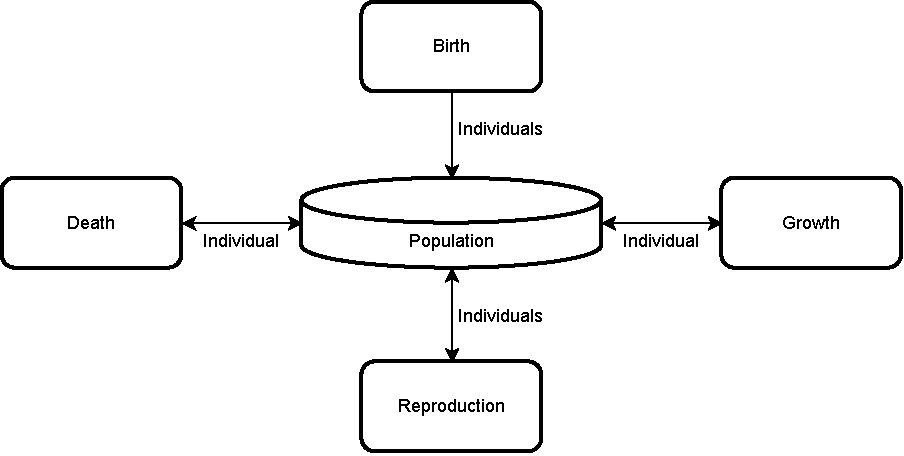
\includegraphics[width=0.90\linewidth]{img/fig_algorithm_model.pdf}
        \caption{General model concept for the Animal Life Cycle Algorithm (ALCA)\cite{Felix-Saul2023}.} \label{fig.algorithm_model}
        \end{figure}


\section{Proposal}
    \label{section.proposal}

    Let's imagine that the colors black and white fell in love and had children. If we had to guess what color their offspring would be, it could only be predictable its children's color would be inside the domain shown in Figure~\ref{fig.grayscale_continuous}.

    \begin{figure}[!ht]
        \centering
        
\includegraphics[width=0.80\linewidth]{img/fig_grayscale_continuous.pdf}
        \caption{Black and white offspring, predictable color domain.} \label{fig.grayscale_continuous}
        \end{figure}

    If we replace the colors black and white with values 0 and 1, respectively, how many values can we find in between? We could replace attributes, switching from color to height, strength, agility, or any other feature we might need to focus on. The parents' attribute values will determine how their offspring's attributes are defined. This paper focuses on breeding (or reproduction), whereas in earlier versions of the algorithm, we used the traditional (GA) one-point crossover. 

    \subsection{Crossover Proposal}

    In this document, we propose a different technique to the canonical approach One Point Crossover, where part of the genetic information is copied directly to each offspring in the crossover operator. This type of crossover may fail to perform successfully in continuous optimization problems. Figure~\ref{fig.onepoint_crossover} provides an example of the One Point Crossover.

    \begin{figure}[!ht]
        \centering
        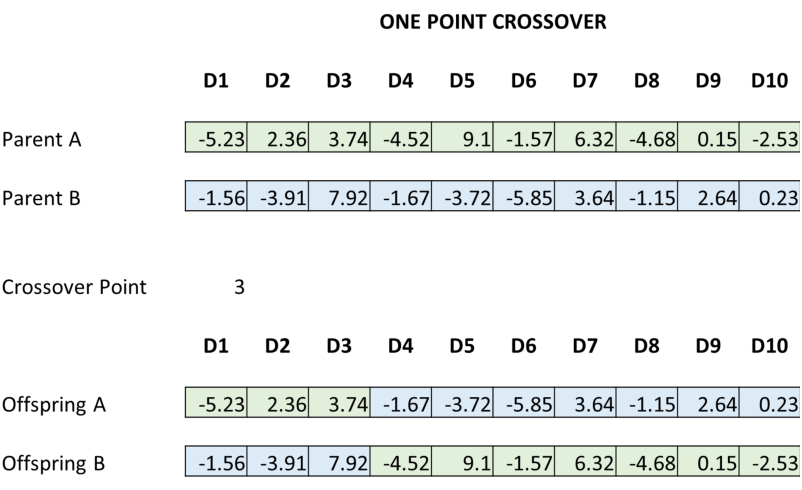
\includegraphics[width=0.90\linewidth]{img/fig_onepoint_crossover.pdf}
        \caption{Classical approach example for the One Point Crossover, with crossover point 3.} \label{fig.onepoint_crossover}
        \end{figure}

    In this proposal, we use the parent's genetic information for each gene, using those values as lower and upper bounds of a range, where a random value within that range determines the new value for that gene index of the offspring. Our proposal example for the Continuous Range Crossover is displayed in Figure~\ref{fig.contrange_crossover}, where it should be noted that we construct a template that will be used for all the offspring generated by each couple.

    An exciting functionality of this strategy is that this new crossover operation will enable the offspring to continue exploring new search spaces with the birth of unique individuals. Because of the new values obtained within the parent's chromosome ranges, this technique will be helpful to avoid local optima stagnation by maintaining diversity due to the near-infinite possibility of stochastic values.

    Our proposed strategy is beneficial for evolutionary algorithms, where the individual's genetic code (or a similar data layout) is the main structure for storing the population information. It could also be valuable for other algorithms, such as Particle Swarm Optimization (PSO), in computing the new placement position caused by the movement of the particles.

    \begin{figure}[!ht]
        \centering
        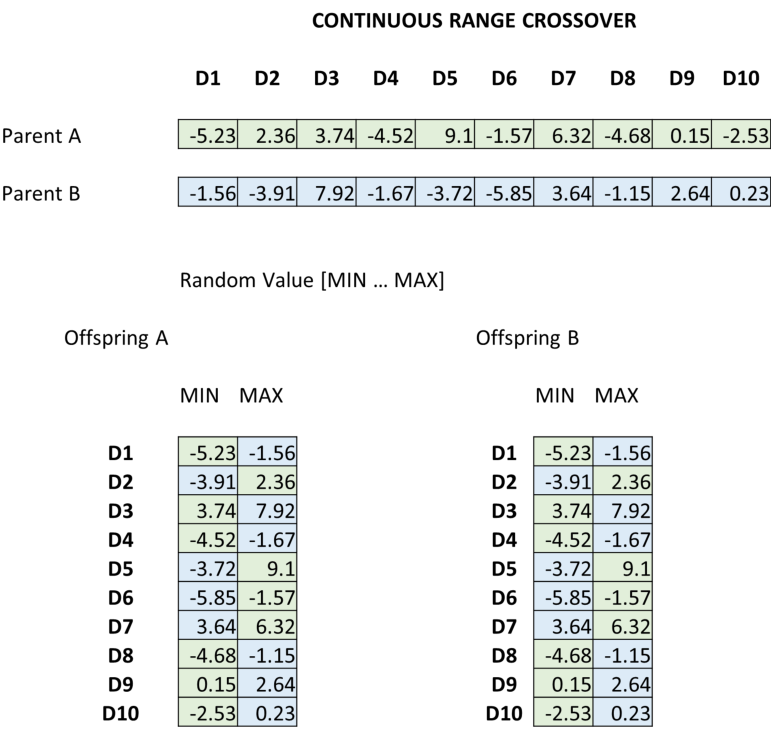
\includegraphics[width=0.90\linewidth]{img/fig_contrange_crossover.pdf}
        \caption{Our proposal example for the Continuous Range Crossover mating the same couple of individuals.} \label{fig.contrange_crossover}
        \end{figure}        
    
    \FloatBarrier

    As shown in Figure~\ref{fig.contrange_crossover}, Continuous Range Crossover, we generate a template with the chromosome values of the parents. We use this template for the generation of all their children. In the following experiment results shown in this document, we have generated two children per couple reproduction, the same way the One Point Crossover strategy does. This offspring number generated has the purpose of maintaining a balance in the population created by the reproduction operator in both proposals.

\section{Experiments}
    \label{section.experiments}

    To validate our proposal, we performed experiments using the mathematical benchmark functions introduced in the Competition on Evolutionary Computation\cite{awad2016problem} for the 2017 edition (CEC-2017) for evaluation to compare the traditional one-point crossover and our proposed strategy. We finalize with a statistical Z-Test with a ninety-five percent confidence level to determine the best alternative. These benchmark functions include shifted and rotated versions of traditional benchmark functions (F1-F10), furthermore, there are ten hybrid versions combining the previous functions (F11-F20). The last functions (F21-30) include several compositions of previous benchmark functions, these are the most difficult variants. 

    We can find a detailed description of the CEC-2017 mathematical benchmark functions, their equations, graphs, and classification in the document \textit{"Problem Definitions and Evaluation Criteria for the CEC 2017 Special Session and Competition on Single Objective Real-Parameter Numerical Optimization"} \cite{awad2016problem}.


    \subsection{Experimental Configuration}

    We used the Animal Life Cycle Algorithm (ALCA) for our experiments, switching between the breeding strategies (One Point and Continuous Range Crossover) with the same general setup. Table~\ref{tab.general_configuration} displays the General Configuration used to run the experiments for our research, where all the values remained consistent during all the stages of the test runs.

    For each of the thirty mathematical benchmark functions from the CEC-2017, we evaluated the ten and thirty dimensions, where we performed fifty-one runs per dimension. To find and determine the best alternative finalized with a statistical Z-Test with a ninety-five percent confidence level.

    \begin{table}[]
    \scriptsize
    \centering
    \caption{Animal Life Cycle Algorithm (ALCA) General Configuration.}\label{tab.general_configuration}    
    \begin{tabular}{@{}ll@{}}
    \toprule
    \multicolumn{2}{l}{\textbf{ALCA   General Configuration}} \\ \midrule
    \textbf{Dimensions Evaluated} & \textbf{10, 30} \\
    Population' Individuals & 500 \\
    Maximum Evaluations & 10,000 * Dim \\
    Rate for Crossover & 100 \\
    Rate for Mutation & 7 \\
    Maximum Age & 5 \\
    Rate for Tournament & 100 \\
    Size of Sample & 20 \\
    Minimum Approval & 80 \\
    Maximum Approval & 200 \\ \bottomrule
    \end{tabular}
    \end{table}

    \FloatBarrier


    \subsection{Experimental Results}

    We describe how to interpret the results presented in our Box and Whisker charts for each mathematical function. For these experiments, we choose to test the benchmark functions with ten and thirty dimensions, while there are higher dimensions, these two present enough challenges to the algorithms to compare the search performance in this kind of problem. According to the rules of the CEC 2017 Benchmark, the number of runs must be 51. The results in the table are then the box plot showing the median of the 51 runs. In green color, we show the results of the canonical One Point crossover found in the original version of GAs, on the right side, in blue color we show the results of our current proposal, the Continuous Range crossover. Because the goal is to minimize the functions, the closer the error values are to the zero value, the better. Below, we describe Figure~\ref{fig.experiment_F1-F5}, which includes functions F1 to F5.  In function F1 for the 10-dimension difficulty, the Continuous Range Crossover (CRx) methodology outperformed the One Point Crossover (OPx) methodology in the statistical test. On the other hand, we needed to find more evidence for thirty dimensions to determine whether any crossover alternative would be better. In the F2 function, for 10 dimensions, again, our proposed approach outperformed the OPx. Moreover, for function F3 for both dimensions, the statistical test found better results for our proposed CRx strategy. At function F4, only for the 10-dimensional problem, the CRx strategy turned out to be better through the statistical test, while for 30 dimensions, there was not a statistically clear winner. Finally, for F5, the statistical test passed only in 10 dimensions.

    We now describe the results for the next set of functions shown in Figure~\ref{fig.experiment_F6-F10}, including functions F6 through F10. In function F6, only for the 30-dimension difficulty, the canonical OPx alternative surpassed our proposal in the statistical test for the first occasion. On the following function, F7, only for the 10-dimension, our proposed CRx outperforms its alternative through the statistical test. Moreover, for functions F8 and F9 for both dimensions, the statistical test found better results for our proposed CRx strategy. For the function F10, the opposite of the previous function occurred, where for both dimensions, the classic OPx strategy obtained better results than our proposal. We describe the results in Figure~\ref{fig.experiment_F11-F15}, including functions F11 through F15. At function F11, only for the 10-dimension, the original OPx passed the statistical test compared to our proposed strategy. For function F12, the CRx strategy found better results for both tested dimensions than the canonical alternative, passing the statistical test. Our proposed strategy proved a better alternative for the F13, F14, and F15 functions at the 30 dimensions test run. We continue describing the results shown in Figure~\ref{fig.experiment_F16-F20}, which includes functions F16 to F20. At function F16, both alternatives obtained similar results on tested dimensions. While for function F17 only for the 10-dimension, our proposed strategy proved better. On the other hand, at functions F18 and F19, only at the 30-dimension test, our proposed CRx passed the statistical test. Finally, for function F20, both crossover alternatives tested equivalent results.

    We continue with the description for the following set of functions shown in Figure~\ref{fig.experiment_F21-F25}, which includes functions F21 through F25. Results obtained at F21 show that only at 30 dimensions did our proposed strategy prove statistically better. Where at F22 on the 10-dimension, the original OPx was the best, for the 30-dimension, our proposed CRx was declared the winner. On the next F23, the OPx proved better for both tested dimensions. At function F24, on the lower 10-dimension, the CRx was a clear victor, while at the 30-dimension, the original OPx was the most precise. The canonical strategy was the most suitable alternative for the last test operation, F25, only at the 30-dimension. We finalize with the description for our last set of functions shown in Figure~\ref{fig.experiment_F26-F30}, which includes functions F26 through F30. The statistical test found no clear winner for the crossover alternatives at the mathematical evaluations, F26, F27, and F29. On the other hand, at operation F28, the proposed CRx statistically overcomes the canonical strategy for both tested dimensions. Lastly, at F30, our proposed CRx was the best alternative for the 30-dimension test.


\section{Discussion}
    \label{section.discussion}

    For our experimentation, we executed fifty-one independent runs per specified dimension for each CEC-2017 mathematical benchmark function. We registered the following values: best-found error average and standard deviation to calculate the statistical Z-Test value. We summarized our results in the following tables, with the labels described next:

    \begin{itemize}
        \item   Fx:          is the mathematical benchmark function.
        \item   Mean:        is the average of the best-found error.
        \item   St-Dev:      is the computed error standard deviation. 
        \item   Z:           is the calculated statistical Z-Test value.
    \end{itemize}

    To find and determine the best alternative, finalized with a statistical Z-Test with a ninety-five percent confidence level. Here are the results' statistics values: Table~\ref{tab.condensed_evaluation_10D} shows the condensed ALCA evaluation results for the CEC-2017 functions running on ten dimensions (D) for alternatives One Point and Continuous Range crossover; Table~\ref{tab.condensed_evaluation_30D} displays the condensed ALCA evaluation results for the CEC-2017 mathematical operations running on thirty D for the same crossover alternatives.

    \begin{table}[]
    \scriptsize
    \centering
    \caption{Condensed ALCA evaluation results for the CEC-2017 functions running on ten dimensions for alternatives One Point and Continuous Range crossover.}\label{tab.condensed_evaluation_10D}    
    \begin{tabular}{@{}cllllllll@{}}
    \toprule
    \multicolumn{9}{c}{\textbf{ALCA   . CEC-2017 Benchmark Functions . 10 Dim}} \\ \midrule
    \textbf{Crossover} & \textbf{} & \multicolumn{3}{c}{\textbf{One Point   Xover}} & \multicolumn{1}{c}{\textbf{}} & \multicolumn{3}{c}{\textbf{Cont. Range   Xover}} \\
    Fx &  & \multicolumn{1}{c}{Mean} & \multicolumn{1}{c}{Std. Dev.} & \multicolumn{1}{c}{Z} & \multicolumn{1}{c}{} & \multicolumn{1}{c}{Mean} & \multicolumn{1}{c}{Std. Dev.} & \multicolumn{1}{c}{Z} \\
    F1 &  & 2.1389E+03 & 2.1399E+03 & 5.4192E+00 &  & 4.4273E+02 & 6.4605E+02 & \textbf{-5.4192E+00} \\
    F2 &  & 1.8100E-03 & 2.6299E-03 & 2.3752E+00 &  & 8.5385E-04 & 1.1614E-03 & \textbf{-2.3752E+00} \\
    F3 &  & 4.1859E-04 & 1.1643E-03 & 2.4856E+00 &  & 1.3284E-05 & 2.1996E-05 & \textbf{-2.4856E+00} \\
    F4 &  & 6.0009E+00 & 1.3061E+01 & 1.9980E+00 &  & 2.3131E+00 & 1.7796E+00 & \textbf{-1.9980E+00} \\
    F5 &  & 1.5256E+01 & 7.0569E+00 & 2.4517E+00 &  & 1.2447E+01 & 4.1425E+00 & \textbf{-2.4517E+00} \\
    F6 &  & 6.0531E-04 & 9.2170E-04 & -1.4267E+00 &  & 2.5341E-03 & 9.6104E-03 & 1.4267E+00 \\
    F7 &  & 3.1484E+01 & 9.0577E+00 & 2.2567E+00 &  & 2.7585E+01 & 8.3786E+00 & \textbf{-2.2567E+00} \\
    F8 &  & 1.7792E+01 & 7.3832E+00 & 8.0015E+00 &  & 8.6230E+00 & 3.5299E+00 & \textbf{-8.0015E+00} \\
    F9 &  & 2.0213E+01 & 2.2424E+01 & 1.8477E+00 &  & 1.2506E+01 & 1.9608E+01 & \textbf{-1.8477E+00} \\
    F10 &  & 4.9585E+02 & 2.2558E+02 & \textbf{-2.0236E+00} &  & 5.9412E+02 & 2.6338E+02 & 2.0236E+00 \\
    F11 &  & 1.1599E+01 & 6.0084E+00 & \textbf{-2.4372E+00} &  & 1.4872E+01 & 7.4763E+00 & 2.4372E+00 \\
    F12 &  & 1.6980E+04 & 1.9876E+04 & 1.9990E+00 &  & 1.0960E+04 & 8.2128E+03 & \textbf{-1.9990E+00} \\
    F13 &  & 7.3909E+03 & 8.1574E+03 & 1.0784E+00 &  & 5.9436E+03 & 5.0303E+03 & -1.0784E+00 \\
    F14 &  & 3.2387E+02 & 6.0517E+02 & 4.6471E-01 &  & 2.6685E+02 & 6.3381E+02 & -4.6471E-01 \\
    F15 &  & 5.7005E+02 & 1.3121E+03 & 1.2452E+00 &  & 3.0689E+02 & 7.4575E+02 & -1.2452E+00 \\
    F16 &  & 1.5553E+02 & 1.2806E+02 & 5.0519E-01 &  & 1.4323E+02 & 1.1771E+02 & -5.0519E-01 \\
    F17 &  & 3.1678E+01 & 3.6537E+01 & 1.8131E+00 &  & 2.1124E+01 & 1.9819E+01 & \textbf{-1.8131E+00} \\
    F18 &  & 2.2591E+03 & 2.8803E+03 & 9.0297E-01 &  & 1.7279E+03 & 3.0584E+03 & -9.0297E-01 \\
    F19 &  & 1.8843E+03 & 3.2365E+03 & 4.1079E-01 &  & 1.6323E+03 & 2.9529E+03 & -4.1079E-01 \\
    F20 &  & 9.5026E+00 & 8.3167E+00 & -1.3542E+00 &  & 1.1957E+01 & 9.9176E+00 & 1.3542E+00 \\
    F21 &  & 1.1492E+02 & 3.8643E+01 & 4.9288E-02 &  & 1.1455E+02 & 3.5773E+01 & -4.9288E-02 \\
    F22 &  & 1.0005E+02 & 2.0717E+01 & \textbf{-2.5672E+00} &  & 1.0813E+02 & 8.6974E+00 & 2.5672E+00 \\
    F23 &  & 3.2068E+02 & 7.3128E+00 & \textbf{-2.5291E+00} &  & 3.2476E+02 & 8.9080E+00 & 2.5291E+00 \\
    F24 &  & 3.2831E+02 & 8.0609E+01 & 5.3612E+00 &  & 2.1484E+02 & 1.2786E+02 & \textbf{-5.3612E+00} \\
    F25 &  & 4.3486E+02 & 2.6137E+01 & 1.3872E+00 &  & 4.2795E+02 & 2.4061E+01 & -1.3872E+00 \\
    F26 &  & 3.9878E+02 & 1.2472E+02 & 7.5476E-01 &  & 3.8231E+02 & 9.3517E+01 & -7.5476E-01 \\
    F27 &  & 3.8835E+02 & 1.0299E+01 & -5.4299E-01 &  & 3.8951E+02 & 1.1293E+01 & 5.4299E-01 \\
    F28 &  & 4.1119E+02 & 7.9226E+01 & 1.9297E+00 &  & 3.7987E+02 & 8.4606E+01 & \textbf{-1.9297E+00} \\
    F29 &  & 2.9963E+02 & 4.3225E+01 & 7.4383E-01 &  & 2.9396E+02 & 3.3009E+01 & -7.4383E-01 \\
    F30 &  & 3.2080E+02 & 1.5217E+02 & -7.1382E-01 &  & 3.4441E+02 & 1.8071E+02 & 7.1382E-01 \\
    \textbf{Total   (W)} & \multicolumn{1}{c}{\textbf{}} & \multicolumn{2}{c}{\textbf{One Point   Xover}} & \multicolumn{1}{c}{\textbf{4 of 30}} & \multicolumn{1}{c}{\textbf{}} & \multicolumn{2}{c}{\textbf{Cont. Range   Xover}} & \multicolumn{1}{c}{\textbf{12 of 30}} \\ \bottomrule
    \end{tabular}
    \end{table}

    \FloatBarrier

    We performed the statistical Z-Test for both crossover alternatives with a 95 percent confidence level. When the One Point passes the test, the Z value is highlighted in bold on the left column. When the Continuous Range passes the statistical test, the Z value is highlighted in bold on the right column. Where we did not find enough evidence to declare one choice as the best alternative, no value was highlighted.


    \begin{table}[]
    \scriptsize
    \centering
    \caption{Condensed ALCA evaluation results for the CEC-2017 functions running on thirty dimensions for alternatives One Point and Continuous Range crossover.}\label{tab.condensed_evaluation_30D}
    \begin{tabular}{@{}cllllllll@{}}
    \toprule
    \multicolumn{9}{c}{\textbf{ALCA   . CEC-2017 Benchmark Functions . 30 Dim}} \\ \midrule
    \textbf{Crossover} & \textbf{} & \multicolumn{3}{c}{\textbf{One Point   Xover}} & \multicolumn{1}{c}{\textbf{}} & \multicolumn{3}{c}{\textbf{Cont. Range   Xover}} \\
    Fx &  & \multicolumn{1}{c}{Mean} & \multicolumn{1}{c}{Std. Dev.} & \multicolumn{1}{c}{Z} & \multicolumn{1}{c}{} & \multicolumn{1}{c}{Mean} & \multicolumn{1}{c}{Std. Dev.} & \multicolumn{1}{c}{Z} \\
    F1 &  & 4.9221E+03 & 6.2052E+03 & 1.5981E+00 &  & 3.3461E+03 & 3.3306E+03 & -1.5981E+00 \\
    F2 &  & 9.2072E+06 & 4.7678E+07 & 1.3686E+00 &  & 6.9569E+04 & 2.4985E+05 & -1.3686E+00 \\
    F3 &  & 1.1683E+02 & 1.1804E+02 & 4.3284E+00 &  & 4.1582E+01 & 3.8455E+01 & \textbf{-4.3284E+00} \\
    F4 &  & 7.1658E+01 & 3.1444E+01 & -5.2921E-01 &  & 7.4645E+01 & 2.5202E+01 & 5.2921E-01 \\
    F5 &  & 9.3827E+01 & 2.4093E+01 & 4.6068E-01 &  & 9.1790E+01 & 2.0430E+01 & -4.6068E-01 \\
    F6 &  & 4.6723E-03 & 1.0247E-02 & \textbf{-2.4217E+00} &  & 2.2849E-02 & 5.2614E-02 & 2.4217E+00 \\
    F7 &  & 1.5523E+02 & 3.0419E+01 & -3.8825E-01 &  & 1.5772E+02 & 3.4361E+01 & 3.8825E-01 \\
    F8 &  & 9.9361E+01 & 2.4339E+01 & 6.8232E+00 &  & 7.2924E+01 & 1.3162E+01 & \textbf{-6.8232E+00} \\
    F9 &  & 1.3710E+03 & 7.2076E+02 & 4.6028E+00 &  & 8.1853E+02 & 4.6408E+02 & \textbf{-4.6028E+00} \\
    F10 &  & 2.7912E+03 & 5.5872E+02 & \textbf{-2.2216E+00} &  & 3.0169E+03 & 4.6303E+02 & 2.2216E+00 \\
    F11 &  & 7.3052E+01 & 2.7205E+01 & -1.0895E+00 &  & 7.8958E+01 & 2.7541E+01 & 1.0895E+00 \\
    F12 &  & 2.1831E+05 & 1.9392E+05 & 4.6137E+00 &  & 8.7259E+04 & 5.9525E+04 & \textbf{-4.6137E+00} \\
    F13 &  & 1.9452E+04 & 2.7290E+04 & 2.0901E+00 &  & 1.1046E+04 & 8.9591E+03 & \textbf{-2.0901E+00} \\
    F14 &  & 2.2151E+04 & 2.1428E+04 & 2.8255E+00 &  & 1.2691E+04 & 1.0610E+04 & \textbf{-2.8255E+00} \\
    F15 &  & 1.2499E+04 & 1.4069E+04 & 4.9618E+00 &  & 2.3697E+03 & 3.8202E+03 & \textbf{-4.9618E+00} \\
    F16 &  & 1.2641E+03 & 3.4529E+02 & 1.4923E-01 &  & 1.2552E+03 & 2.4941E+02 & -1.4923E-01 \\
    F17 &  & 6.0224E+02 & 1.7565E+02 & 1.1651E+00 &  & 5.5424E+02 & 2.3605E+02 & -1.1651E+00 \\
    F18 &  & 1.2865E+05 & 1.1706E+05 & 2.9170E+00 &  & 7.4398E+04 & 6.2747E+04 & \textbf{-2.9170E+00} \\
    F19 &  & 9.7805E+03 & 1.1607E+04 & 3.0408E+00 &  & 4.3849E+03 & 5.0850E+03 & \textbf{-3.0408E+00} \\
    F20 &  & 4.8317E+02 & 1.6940E+02 & 1.0238E-01 &  & 4.7938E+02 & 2.0307E+02 & -1.0238E-01 \\
    F21 &  & 3.0294E+02 & 2.4353E+01 & 4.3999E+00 &  & 2.8493E+02 & 1.6184E+01 & \textbf{-4.3999E+00} \\
    F22 &  & 1.7571E+03 & 1.7169E+03 & 6.0688E+00 &  & 2.1583E+02 & 5.8436E+02 & \textbf{-6.0688E+00} \\
    F23 &  & 4.6160E+02 & 3.0564E+01 & \textbf{-5.2747E+00} &  & 5.0468E+02 & 4.9672E+01 & 5.2747E+00 \\
    F24 &  & 6.4513E+02 & 7.4299E+01 & \textbf{-2.3148E+00} &  & 6.7829E+02 & 7.0328E+01 & 2.3148E+00 \\
    F25 &  & 3.8492E+02 & 1.4918E+01 & \textbf{-3.0635E+00} &  & 3.9704E+02 & 2.3987E+01 & 3.0635E+00 \\
    F26 &  & 2.3955E+03 & 4.8813E+02 & -1.2340E+00 &  & 2.6143E+03 & 1.1683E+03 & 1.2340E+00 \\
    F27 &  & 4.9415E+02 & 1.2280E+01 & 2.9755E-01 &  & 4.9319E+02 & 1.9531E+01 & -2.9755E-01 \\
    F28 &  & 4.6268E+02 & 4.2897E+01 & 9.2609E+00 &  & 3.9779E+02 & 2.5756E+01 & \textbf{-9.2609E+00} \\
    F29 &  & 9.2249E+02 & 2.3560E+02 & 1.5461E+00 &  & 8.5552E+02 & 2.0043E+02 & -1.5461E+00 \\
    F30 &  & 3.5332E+03 & 4.1540E+03 & 4.0881E+00 &  & 1.0823E+03 & 1.0372E+03 & \textbf{-4.0881E+00} \\
    \textbf{Total   (W)} & \multicolumn{1}{c}{\textbf{}} & \multicolumn{2}{c}{\textbf{One Point   Xover}} & \multicolumn{1}{c}{\textbf{5 of 30}} & \multicolumn{1}{c}{\textbf{}} & \multicolumn{2}{c}{\textbf{Cont. Range   Xover}} & \multicolumn{1}{c}{\textbf{13 of 30}} \\ \bottomrule
    \end{tabular}
    \end{table}

    \FloatBarrier


\section{Conclusions}
    \label{section.conclusions}

    To validate our research, we performed the statistical Z-Test with a ninety-five percent confidence level to analyze the alternatives we present in this proposal. In the ten-dimension category, we found that One Point crossover was the better alternative on four occasions, while our Continuous Range proposal was better on twelve other functions out of thirty. For the thirty-dimensions category, the One Point crossover was better on five occasions, while the Continuous Range crossover was the best alternative on another thirteen. Our experiment results confirm that our solution can be considered an adequate alternative.

    Some researchers might consider our proposal similar to what is used by algorithms such as Differential Evolution, where we consider our proposal to be a variation of existing proposals because we expect this new operator to allow the offspring to continue exploring new search spaces with the birth of individuals. Experimental results indicate that our proposed operator may be a viable alternative for the canonical One Point crossover.

    Based on the analysis of our results, we have shown that the proposed crossover alternative for the reproduction of individuals in a population obtains good results. Therefore, it can be valuable in other evolutionary algorithms where the information of individuals has a structure similar to that of the genetic code. However, with some adaptation, it could be helpful in different types of algorithms, such as Particle Swarm Optimization. In future work, we could investigate a combination between the canonical One Point Crossover strategy and randomly alternating with the proposed Continuous Range Crossover.


\begin{acknowledgement}
    TecNM Project 18186.23-P has partially funded this research.
\end{acknowledgement}

    
    \begin{figure}[!ht]
        \begin{minipage}[h]{0.49\linewidth}
            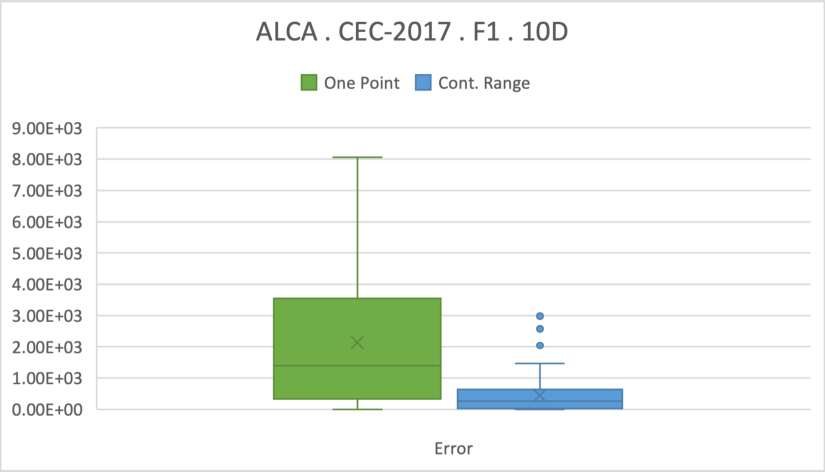
\includegraphics[width=1\linewidth]{img/fig_experiment_F1x10D.pdf} 
        \end{minipage}
        \hfill
        \begin{minipage}[h]{0.49\linewidth}
            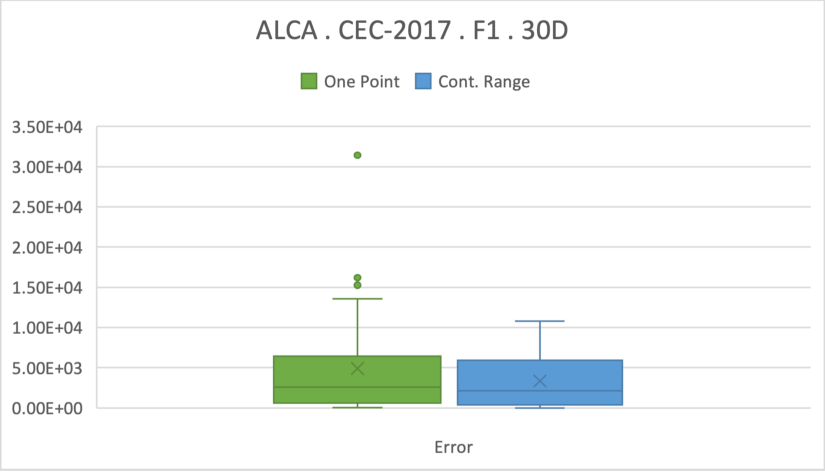
\includegraphics[width=1\linewidth]{img/fig_experiment_F1x30D.pdf} 
        \end{minipage}
        \vfill
        \vspace{0.05 cm}
        \begin{minipage}[h]{0.49\linewidth}
            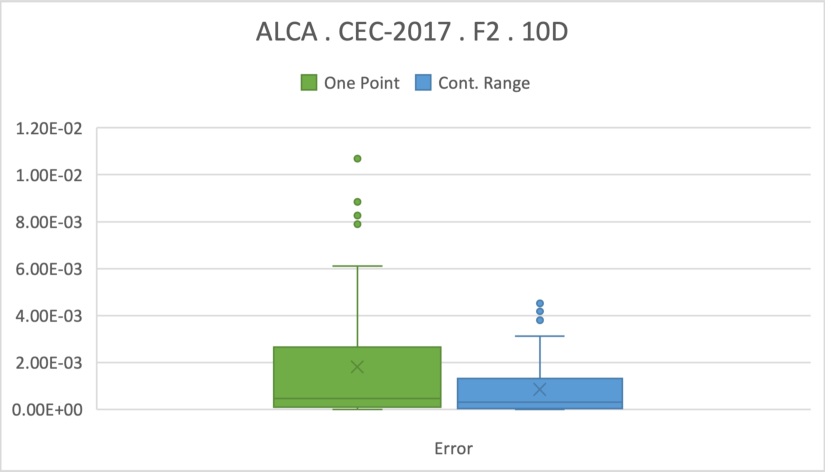
\includegraphics[width=1\linewidth]{img/fig_experiment_F2x10D.pdf} 
        \end{minipage}
        \hfill
        \begin{minipage}[h]{0.49\linewidth}
            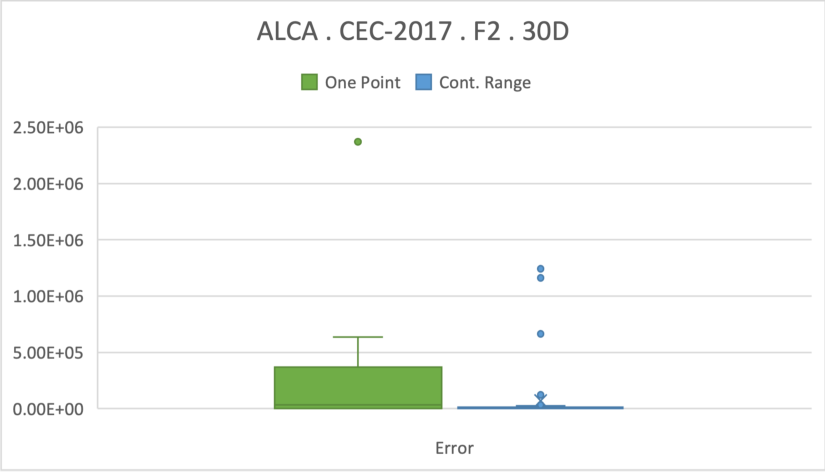
\includegraphics[width=1\linewidth]{img/fig_experiment_F2x30D.pdf} 
        \end{minipage}
        \vfill
        \vspace{0.05 cm}
        \begin{minipage}[h]{0.49\linewidth}
            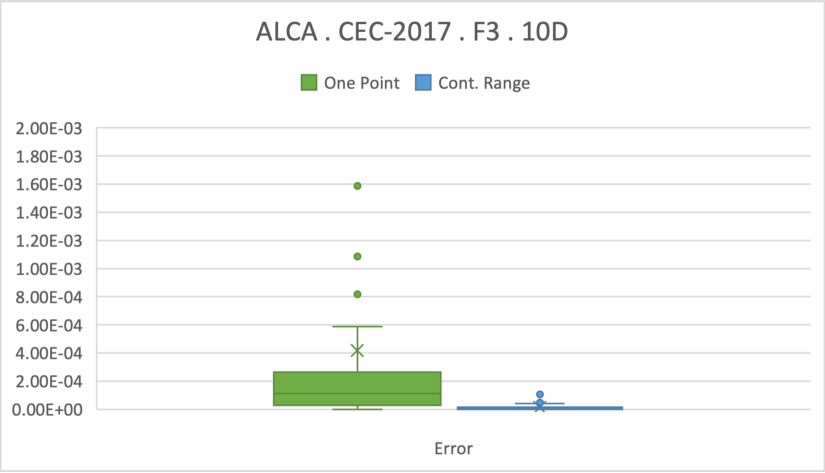
\includegraphics[width=1\linewidth]{img/fig_experiment_F3x10D.pdf} 
        \end{minipage}
        \hfill
        \begin{minipage}[h]{0.49\linewidth}
            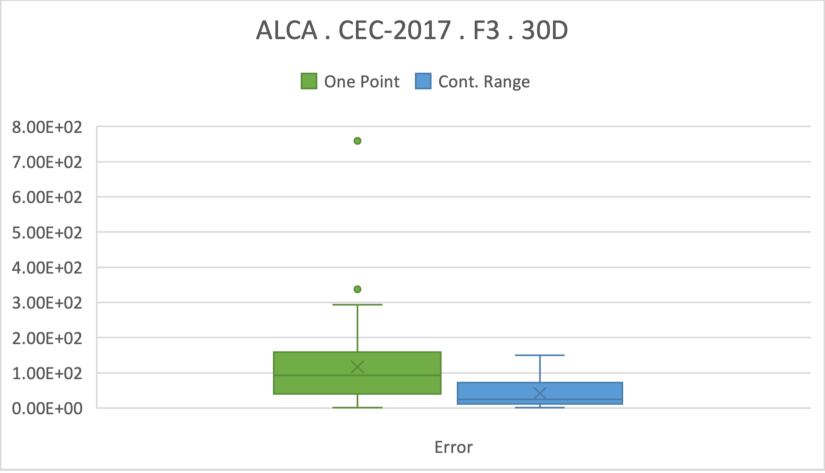
\includegraphics[width=1\linewidth]{img/fig_experiment_F3x30D.pdf} 
        \end{minipage}
        \vfill
        \vspace{0.05 cm}
        \begin{minipage}[h]{0.49\linewidth}
            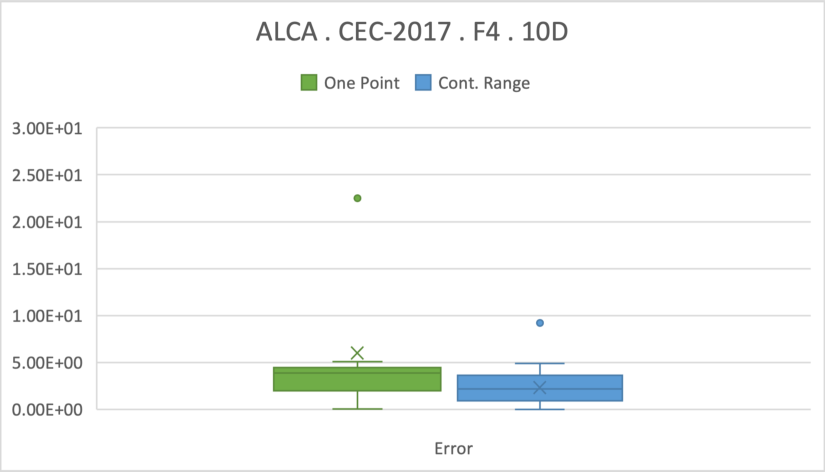
\includegraphics[width=1\linewidth]{img/fig_experiment_F4x10D.pdf} 
        \end{minipage}
        \hfill
        \begin{minipage}[h]{0.49\linewidth}
            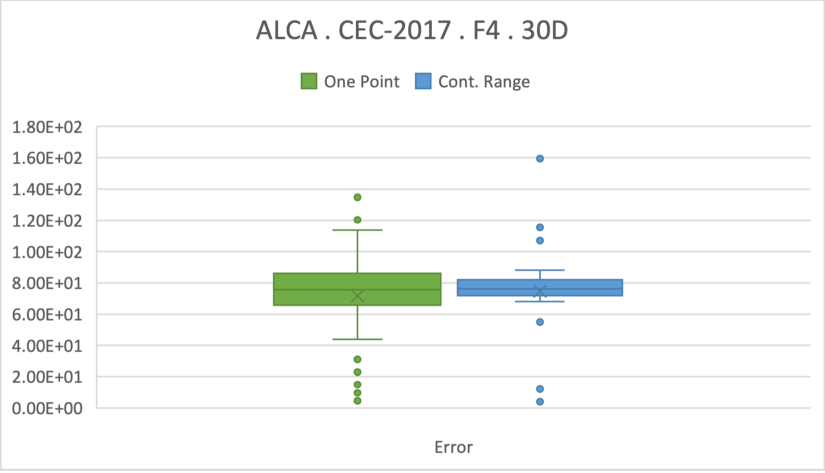
\includegraphics[width=1\linewidth]{img/fig_experiment_F4x30D.pdf} 
        \end{minipage}
        \vfill
        \vspace{0.05 cm}
        \begin{minipage}[h]{0.49\linewidth}
            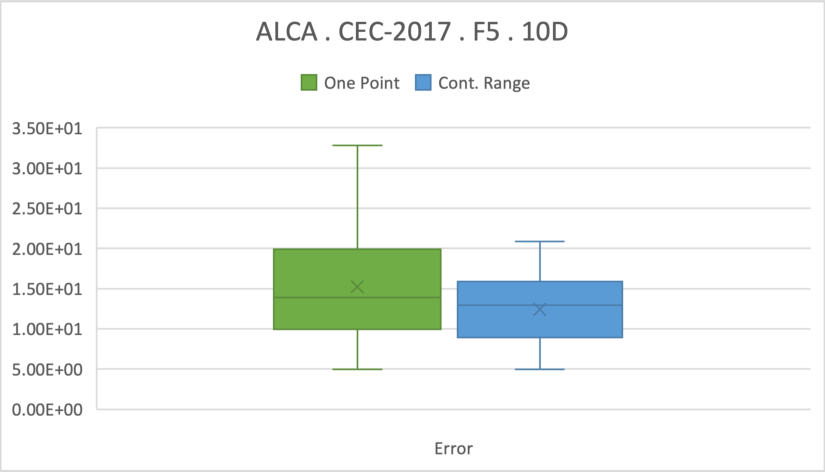
\includegraphics[width=1\linewidth]{img/fig_experiment_F5x10D.pdf} 
        \end{minipage}
        \hfill
        \begin{minipage}[h]{0.49\linewidth}
            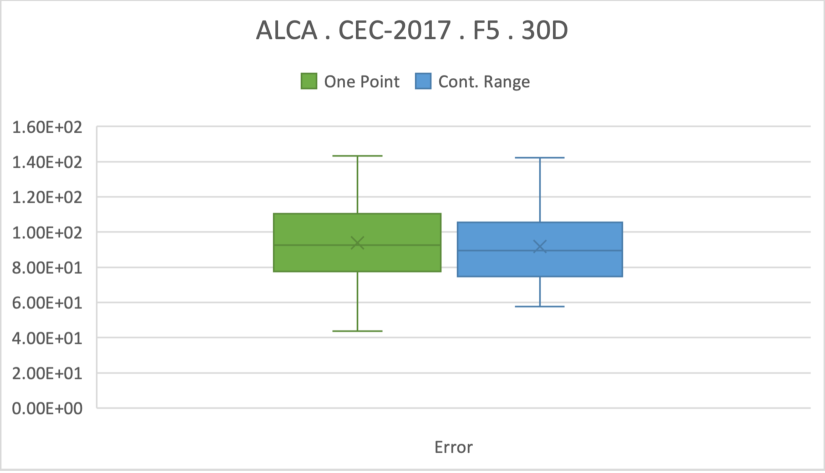
\includegraphics[width=1\linewidth]{img/fig_experiment_F5x30D.pdf} 
        \end{minipage}       
        
        \caption{Box and Whisker charts for mathematical functions F1 to F5. We display the ten and thirty-dimension charts on the left and right sides for the results accumulated in 51 runs.} \label{fig.experiment_F1-F5}
    \end{figure}

    \FloatBarrier

    \begin{figure}[!ht]
        \begin{minipage}[h]{0.49\linewidth}
            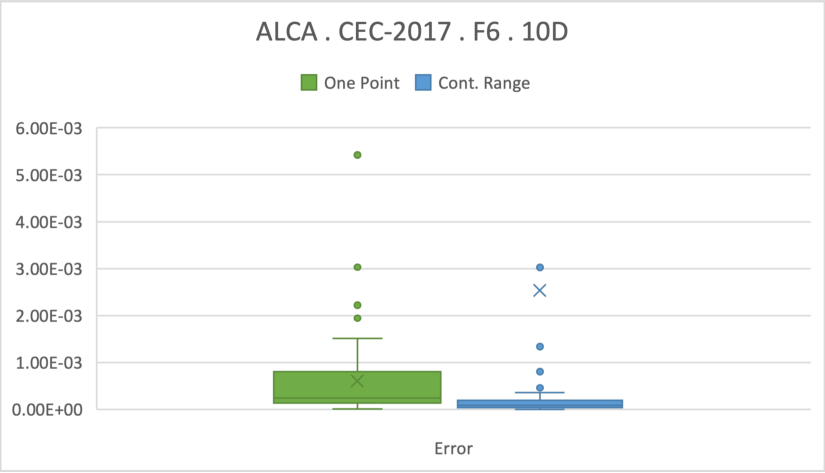
\includegraphics[width=1\linewidth]{img/fig_experiment_F6x10D.pdf} 
        \end{minipage}
        \hfill
        \begin{minipage}[h]{0.49\linewidth}
            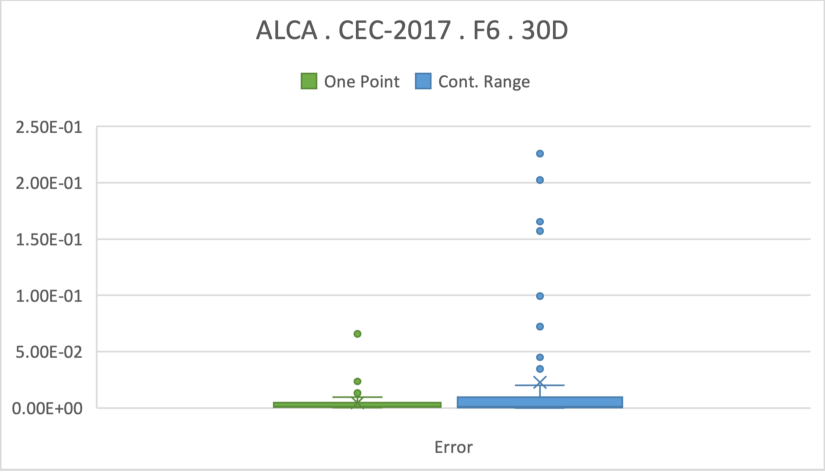
\includegraphics[width=1\linewidth]{img/fig_experiment_F6x30D.pdf} 
        \end{minipage} 
        \vfill
        \vspace{0.05 cm}
        \begin{minipage}[h]{0.49\linewidth}
            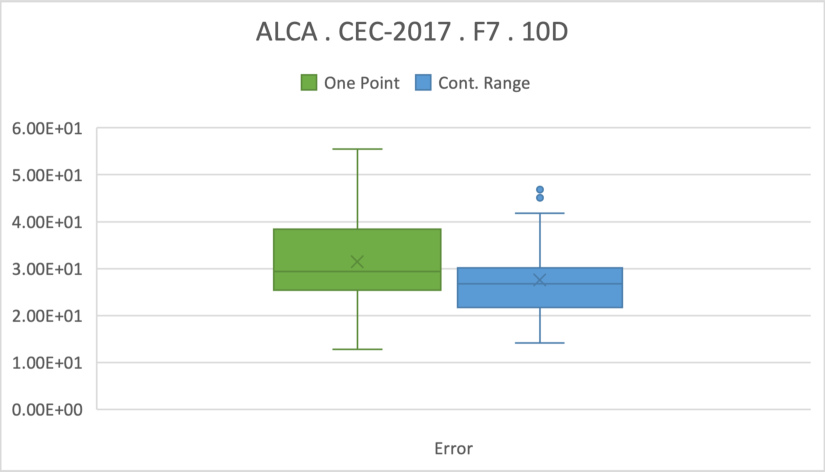
\includegraphics[width=1\linewidth]{img/fig_experiment_F7x10D.pdf} 
        \end{minipage}
        \hfill
        \begin{minipage}[h]{0.49\linewidth}
            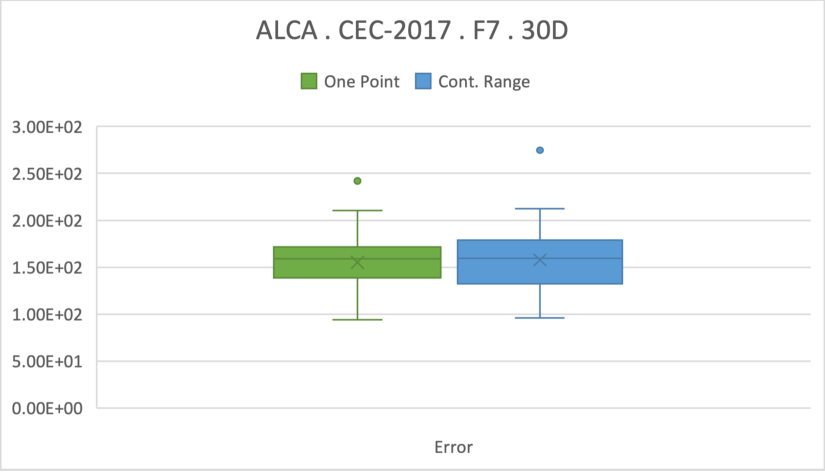
\includegraphics[width=1\linewidth]{img/fig_experiment_F7x30D.pdf} 
        \end{minipage}
        \vfill
        \vspace{0.05 cm}
        \begin{minipage}[h]{0.49\linewidth}
            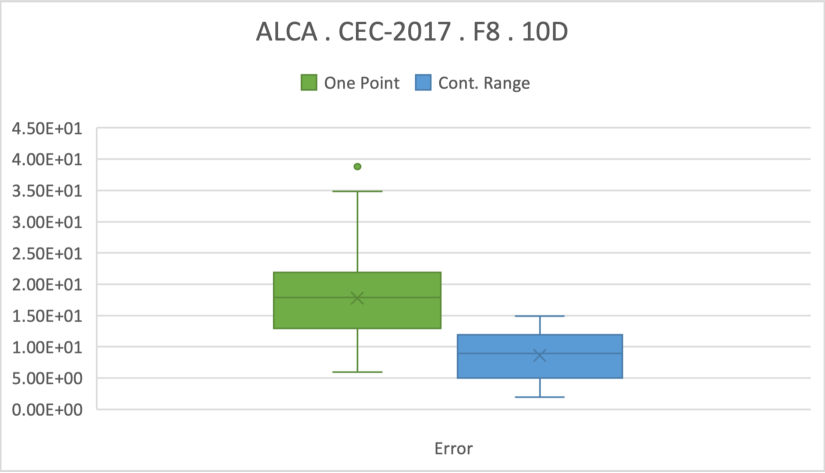
\includegraphics[width=1\linewidth]{img/fig_experiment_F8x10D.pdf} 
        \end{minipage}
        \hfill
        \begin{minipage}[h]{0.49\linewidth}
            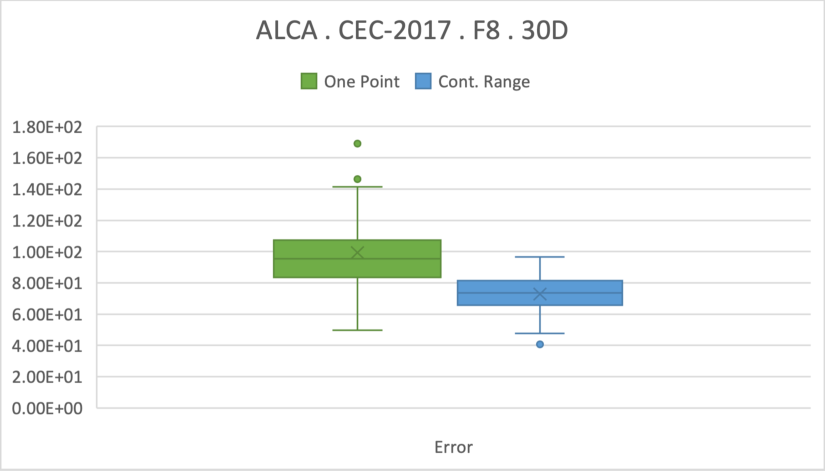
\includegraphics[width=1\linewidth]{img/fig_experiment_F8x30D.pdf} 
        \end{minipage}
        \vfill
        \vspace{0.05 cm}
        \begin{minipage}[h]{0.49\linewidth}
            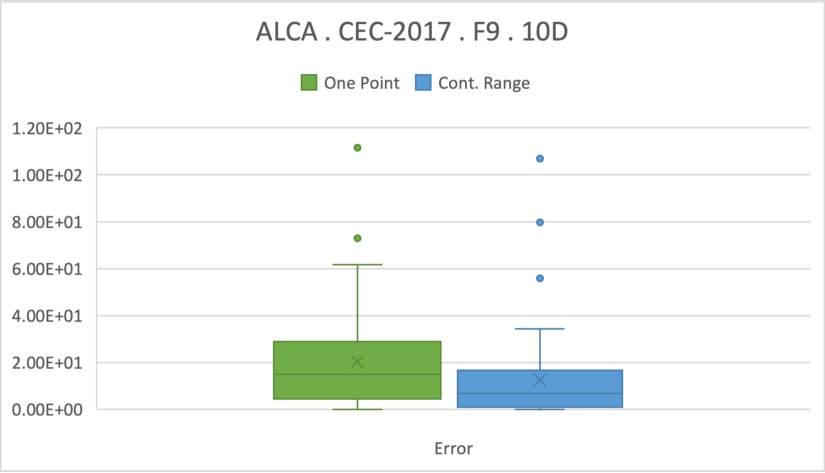
\includegraphics[width=1\linewidth]{img/fig_experiment_F9x10D.pdf} 
        \end{minipage}
        \hfill
        \vspace{0.05 cm}
        \begin{minipage}[h]{0.49\linewidth}
            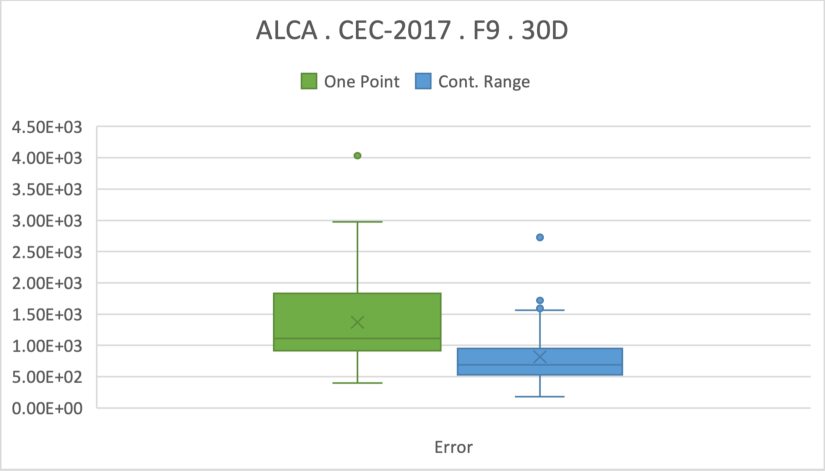
\includegraphics[width=1\linewidth]{img/fig_experiment_F9x30D.pdf} 
        \end{minipage}
        \vfill
        \vspace{0.05 cm}
        \begin{minipage}[h]{0.49\linewidth}
            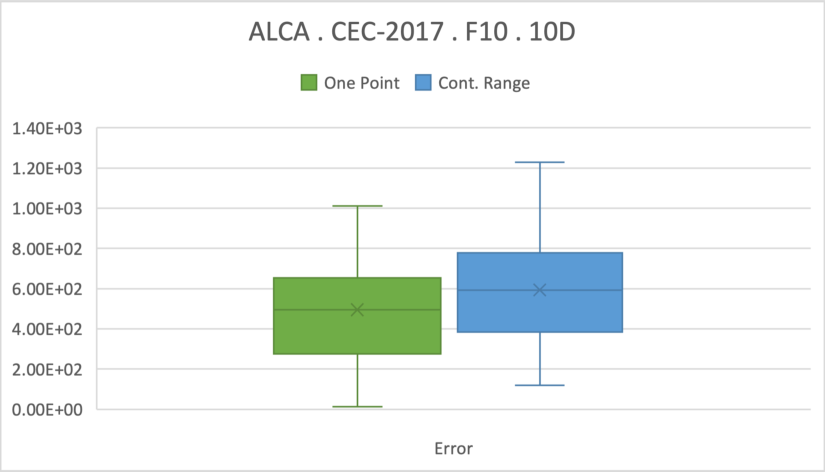
\includegraphics[width=1\linewidth]{img/fig_experiment_F10x10D.pdf} 
        \end{minipage}
        \hfill
        \begin{minipage}[h]{0.49\linewidth}
            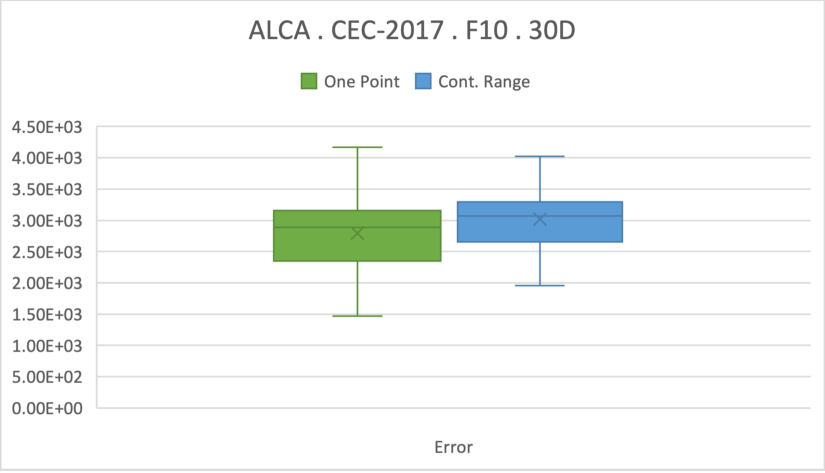
\includegraphics[width=1\linewidth]{img/fig_experiment_F10x30D.pdf} 
        \end{minipage}
        
        \caption{Box and Whisker charts for mathematical functions F6 to F10. We display the ten and thirty-dimension charts on the left and right sides for the results accumulated in 51 runs.} \label{fig.experiment_F6-F10}
    \end{figure}

    \FloatBarrier

    \begin{figure}[!ht]
        \begin{minipage}[h]{0.49\linewidth}
            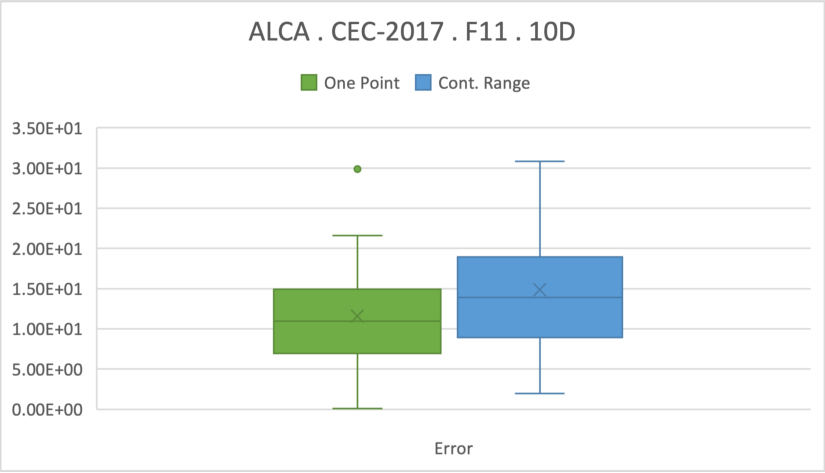
\includegraphics[width=1\linewidth]{img/fig_experiment_F11x10D.pdf} 
        \end{minipage}
        \hfill
        \begin{minipage}[h]{0.49\linewidth}
            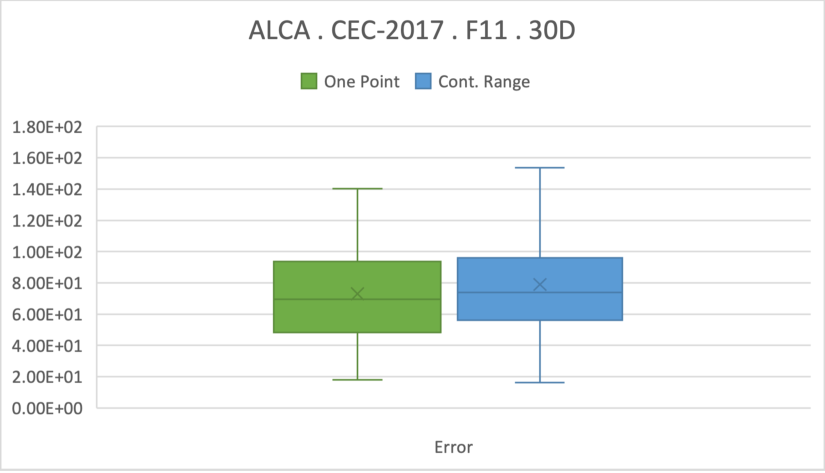
\includegraphics[width=1\linewidth]{img/fig_experiment_F11x30D.pdf} 
        \end{minipage}
        \vfill
        \vspace{0.05 cm}
        \begin{minipage}[h]{0.49\linewidth}
            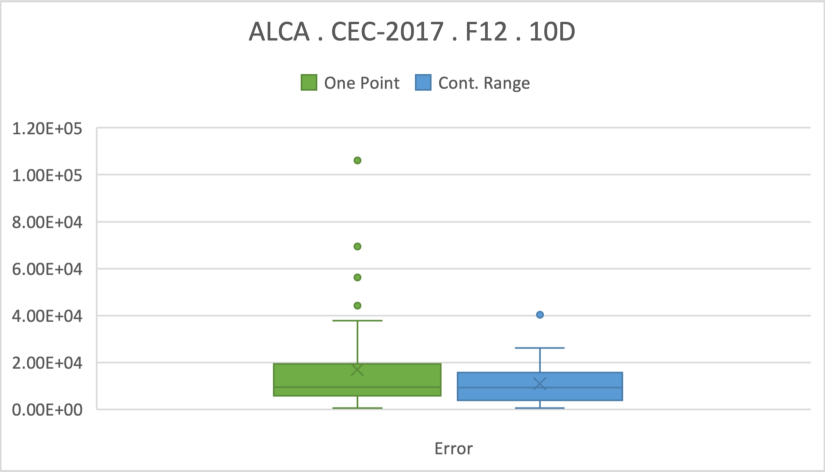
\includegraphics[width=1\linewidth]{img/fig_experiment_F12x10D.pdf} 
        \end{minipage}
        \hfill
        \begin{minipage}[h]{0.49\linewidth}
            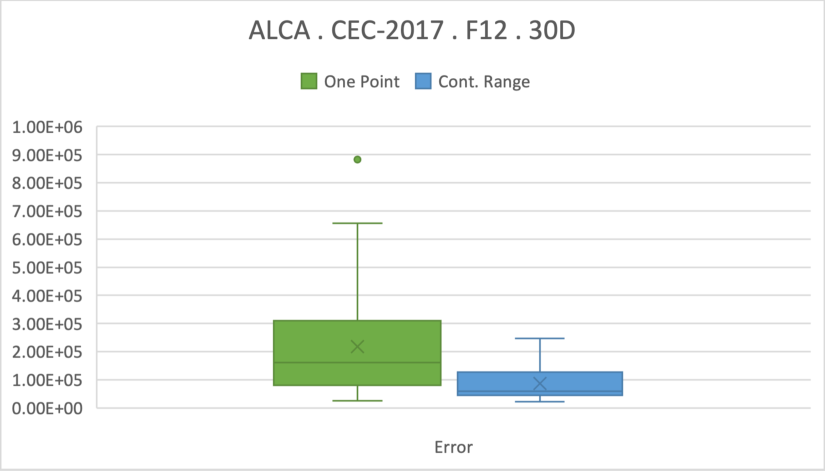
\includegraphics[width=1\linewidth]{img/fig_experiment_F12x30D.pdf} 
        \end{minipage}
        \vfill
        \vspace{0.05 cm}    
        \begin{minipage}[h]{0.49\linewidth}
            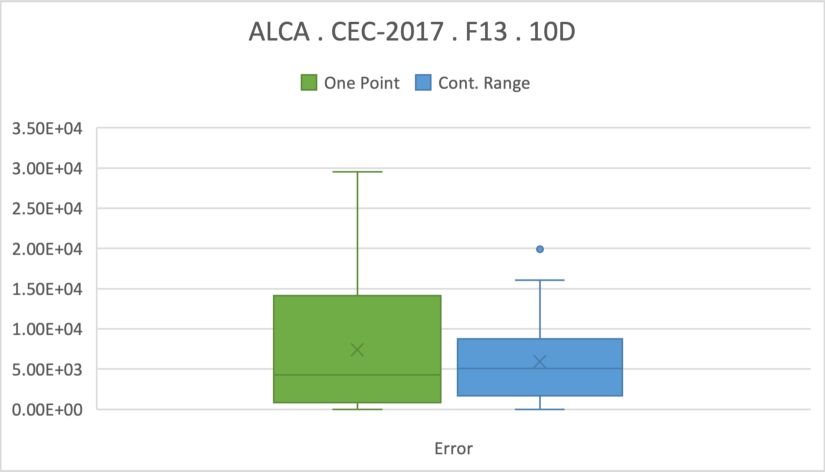
\includegraphics[width=1\linewidth]{img/fig_experiment_F13x10D.pdf} 
        \end{minipage}
        \hfill
        \begin{minipage}[h]{0.49\linewidth}
            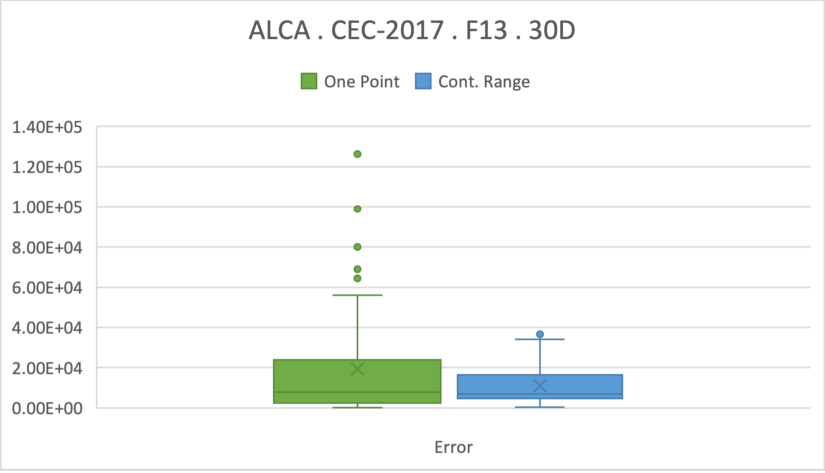
\includegraphics[width=1\linewidth]{img/fig_experiment_F13x30D.pdf} 
        \end{minipage}
        \vfill
        \vspace{0.05 cm}
        \begin{minipage}[h]{0.49\linewidth}
            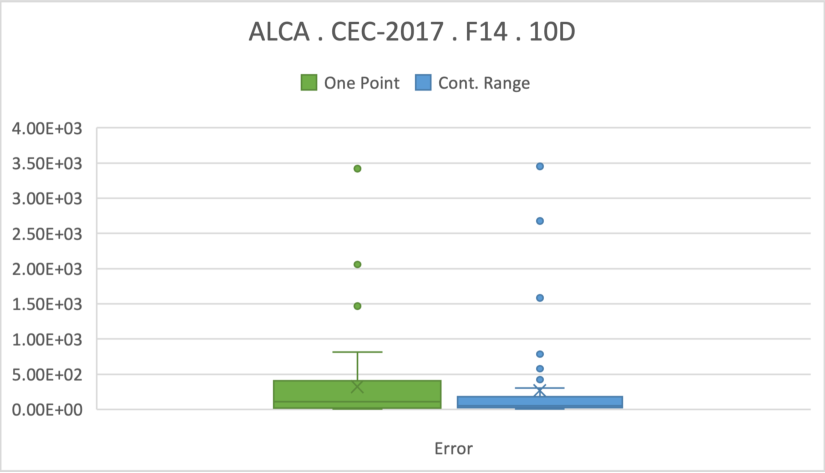
\includegraphics[width=1\linewidth]{img/fig_experiment_F14x10D.pdf} 
        \end{minipage}
        \hfill
        \begin{minipage}[h]{0.49\linewidth}
            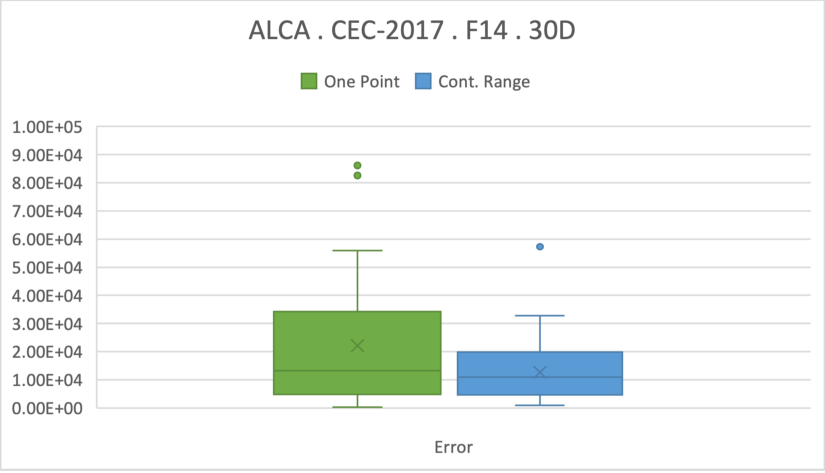
\includegraphics[width=1\linewidth]{img/fig_experiment_F14x30D.pdf} 
        \end{minipage}
        \vfill
        \vspace{0.05 cm}
        \begin{minipage}[h]{0.49\linewidth}
            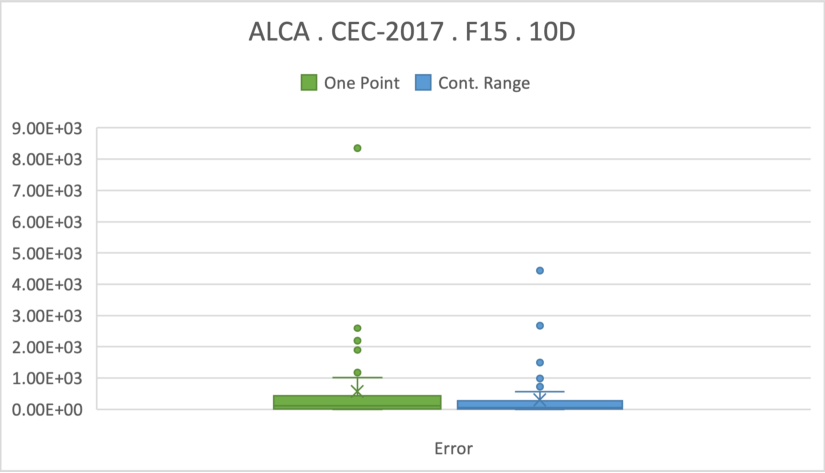
\includegraphics[width=1\linewidth]{img/fig_experiment_F15x10D.pdf} 
        \end{minipage}
        \hfill
        \vspace{0.05 cm}
        \begin{minipage}[h]{0.49\linewidth}
            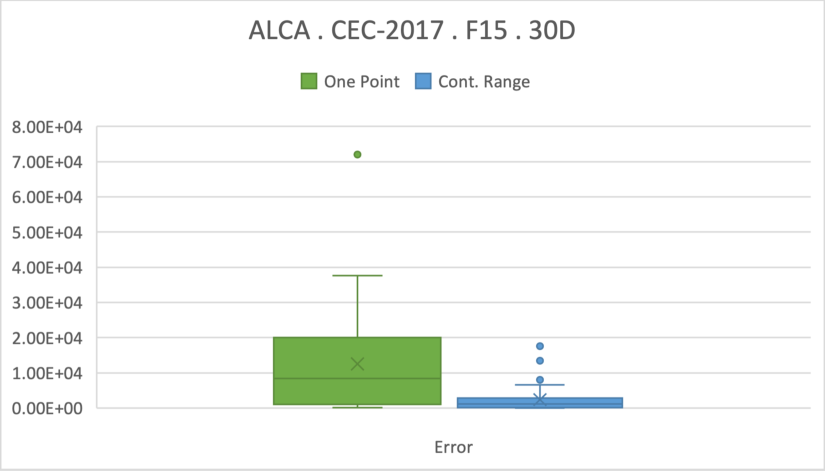
\includegraphics[width=1\linewidth]{img/fig_experiment_F15x30D.pdf} 
        \end{minipage}

        \caption{Box and Whisker charts for mathematical functions F11 to F15. We display the ten and thirty-dimension charts on the left and right sides for the results accumulated in 51 runs.} \label{fig.experiment_F11-F15}
    \end{figure}

    \FloatBarrier

    \begin{figure}[!ht]
        \begin{minipage}[h]{0.49\linewidth}
            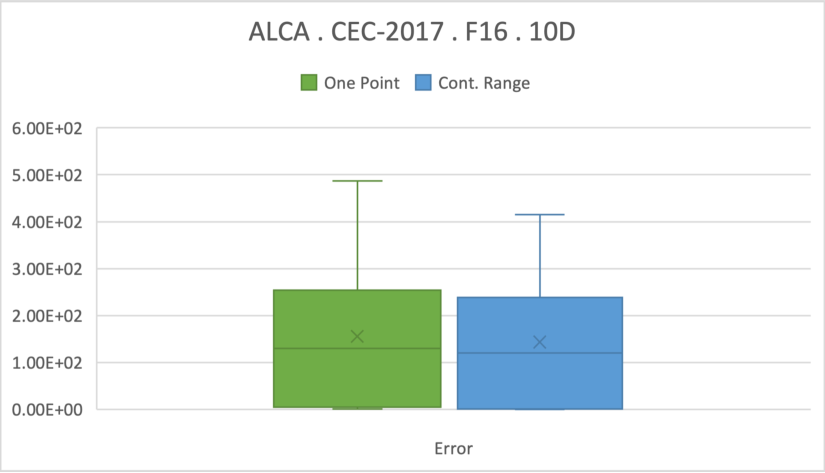
\includegraphics[width=1\linewidth]{img/fig_experiment_F16x10D.pdf} 
        \end{minipage}
        \hfill
        \begin{minipage}[h]{0.49\linewidth}
            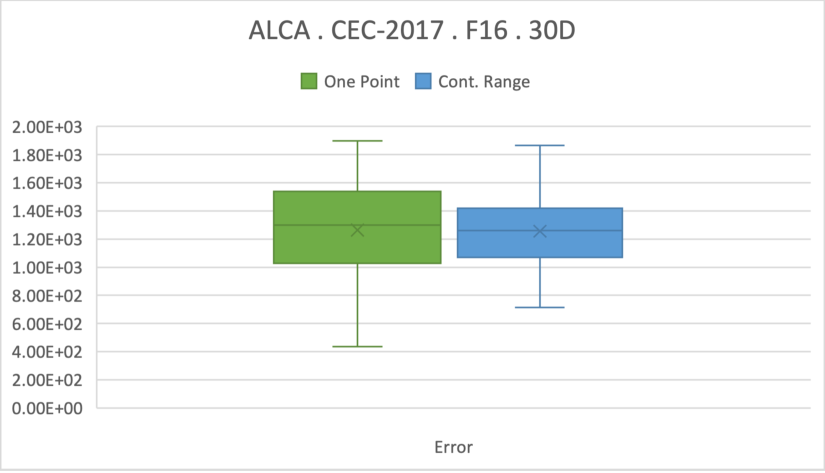
\includegraphics[width=1\linewidth]{img/fig_experiment_F16x30D.pdf} 
        \end{minipage}
        \vfill
        \vspace{0.05 cm}
        \begin{minipage}[h]{0.49\linewidth}
            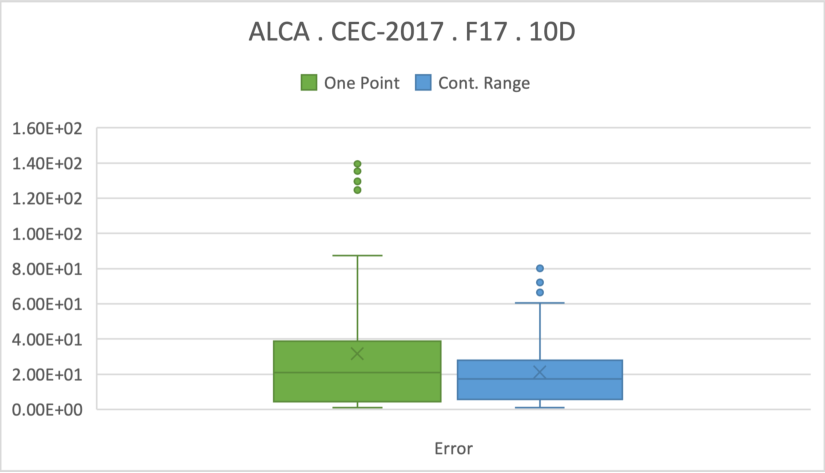
\includegraphics[width=1\linewidth]{img/fig_experiment_F17x10D.pdf} 
        \end{minipage}
        \hfill
        \begin{minipage}[h]{0.49\linewidth}
            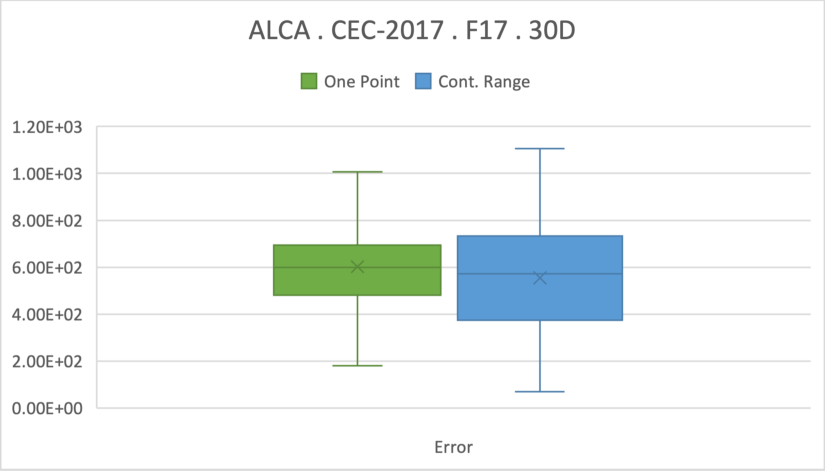
\includegraphics[width=1\linewidth]{img/fig_experiment_F17x30D.pdf} 
        \end{minipage}
        \vfill
        \vspace{0.05 cm}
        \begin{minipage}[h]{0.49\linewidth}
            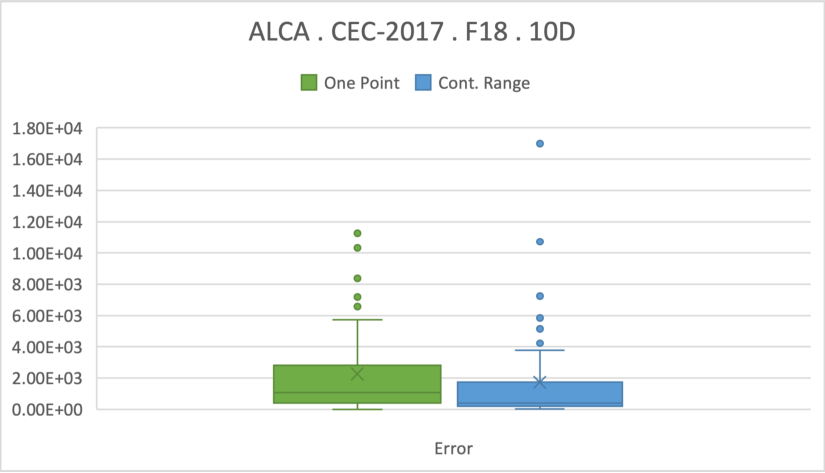
\includegraphics[width=1\linewidth]{img/fig_experiment_F18x10D.pdf} 
        \end{minipage}
        \hfill
        \begin{minipage}[h]{0.49\linewidth}
            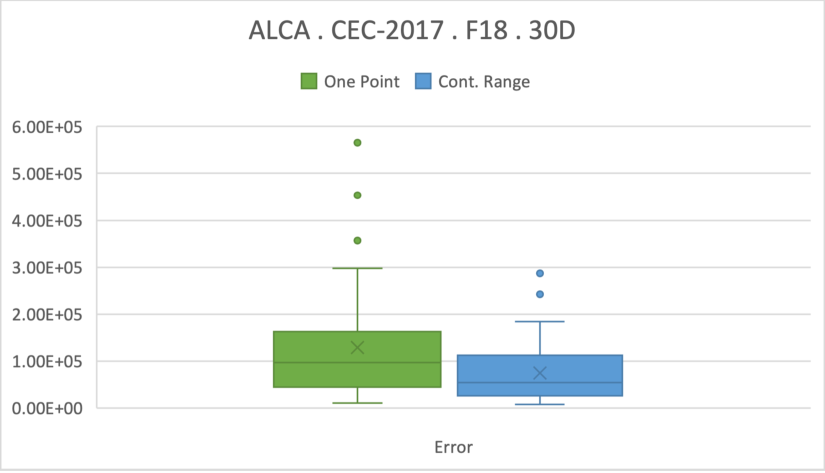
\includegraphics[width=1\linewidth]{img/fig_experiment_F18x30D.pdf} 
        \end{minipage}
        \vfill
        \vspace{0.05 cm}    
        \begin{minipage}[h]{0.49\linewidth}
            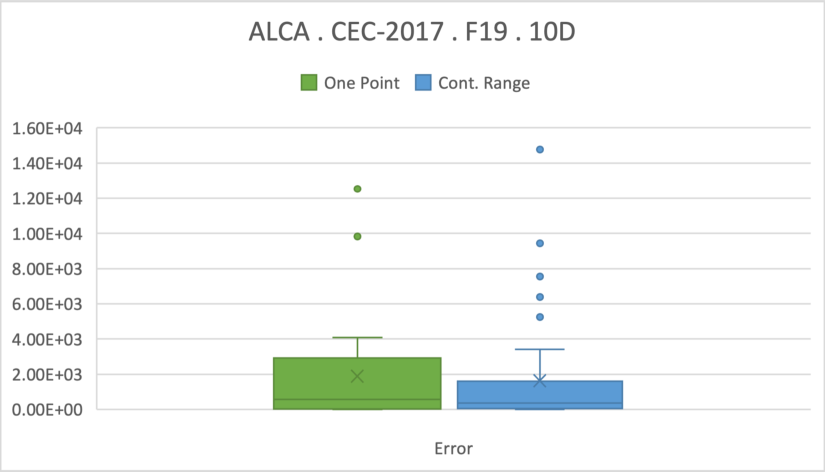
\includegraphics[width=1\linewidth]{img/fig_experiment_F19x10D.pdf} 
        \end{minipage}
        \hfill
        \begin{minipage}[h]{0.49\linewidth}
            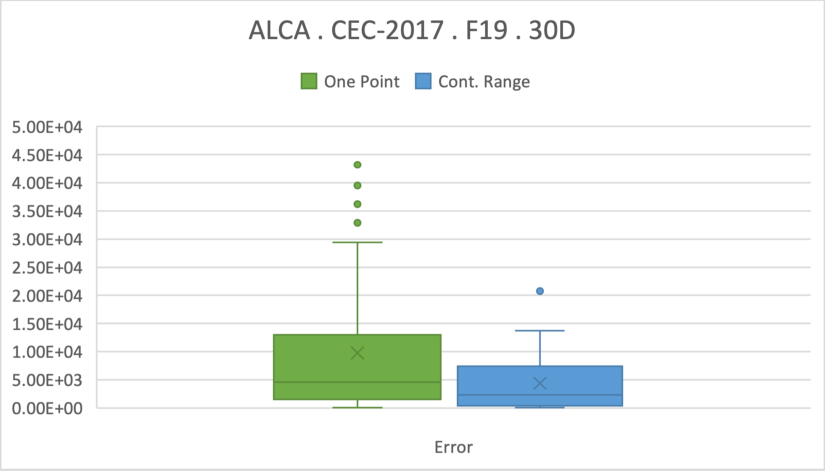
\includegraphics[width=1\linewidth]{img/fig_experiment_F19x30D.pdf} 
        \end{minipage}
        \vfill
        \vspace{0.05 cm}
        \begin{minipage}[h]{0.49\linewidth}
            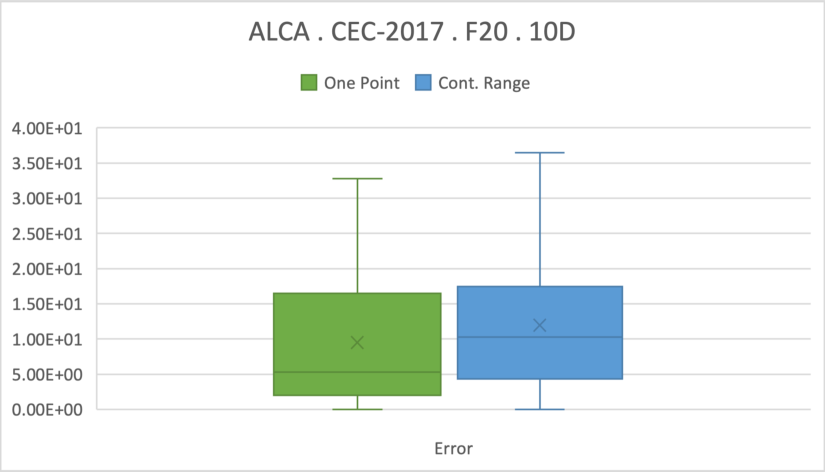
\includegraphics[width=1\linewidth]{img/fig_experiment_F20x10D.pdf} 
        \end{minipage}
        \hfill
        \begin{minipage}[h]{0.49\linewidth}
            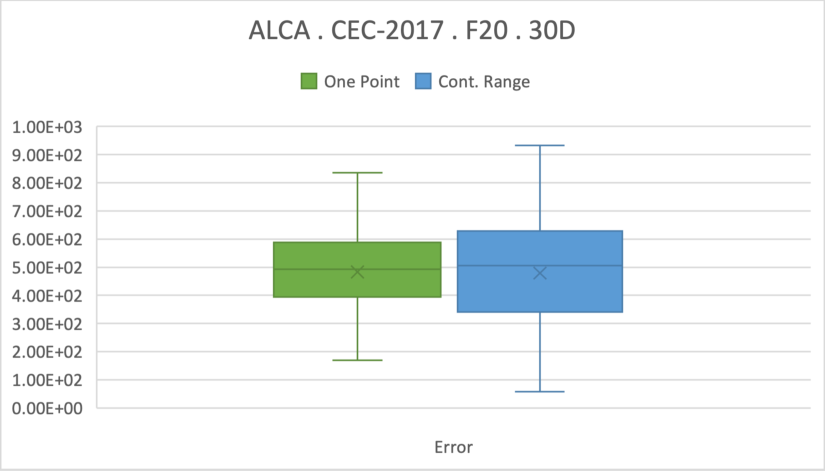
\includegraphics[width=1\linewidth]{img/fig_experiment_F20x30D.pdf} 
        \end{minipage}
        
        \caption{Box and Whisker charts for mathematical functions F16 to F20. We display the ten and thirty-dimension charts on the left and right sides for the results accumulated in 51 runs.} \label{fig.experiment_F16-F20}
    \end{figure}

    \FloatBarrier

    \begin{figure}[!ht]
        \begin{minipage}[h]{0.49\linewidth}
            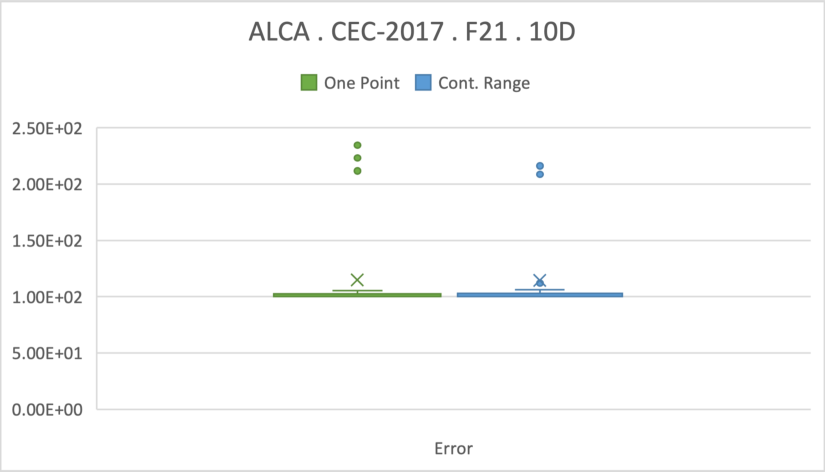
\includegraphics[width=1\linewidth]{img/fig_experiment_F21x10D.pdf} 
        \end{minipage}
        \hfill
        \vspace{0.05 cm}
        \begin{minipage}[h]{0.49\linewidth}
            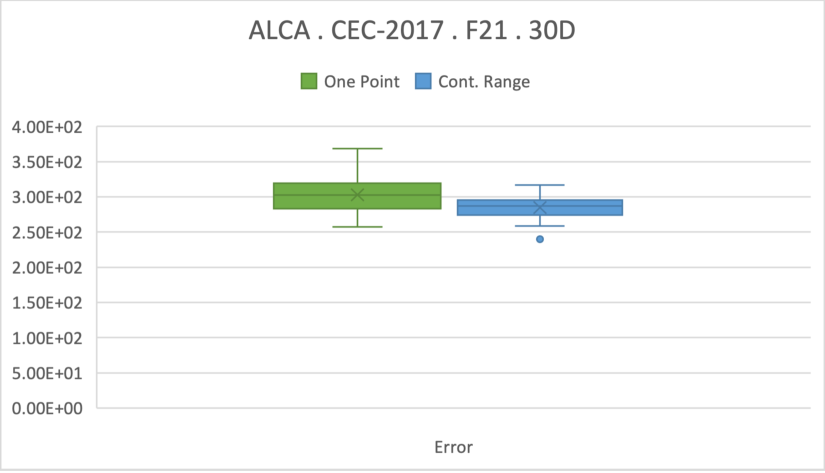
\includegraphics[width=1\linewidth]{img/fig_experiment_F21x30D.pdf} 
        \end{minipage}
        \vfill
        \vspace{0.05 cm}
        \begin{minipage}[h]{0.49\linewidth}
            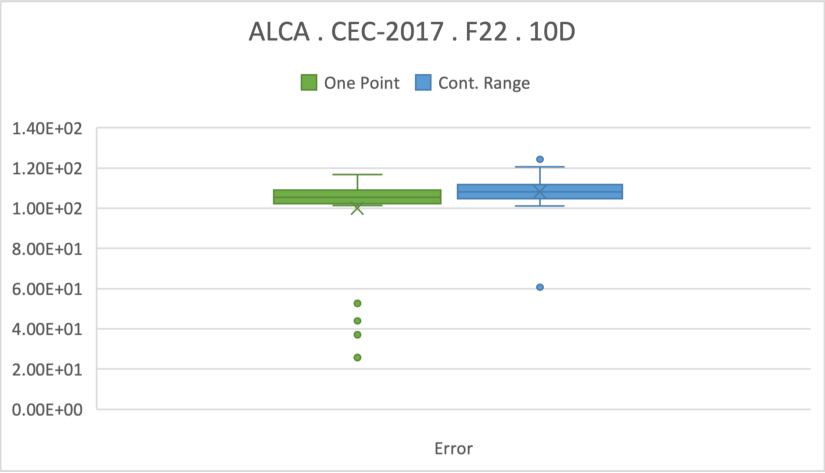
\includegraphics[width=1\linewidth]{img/fig_experiment_F22x10D.pdf} 
        \end{minipage}
        \hfill
        \begin{minipage}[h]{0.49\linewidth}
            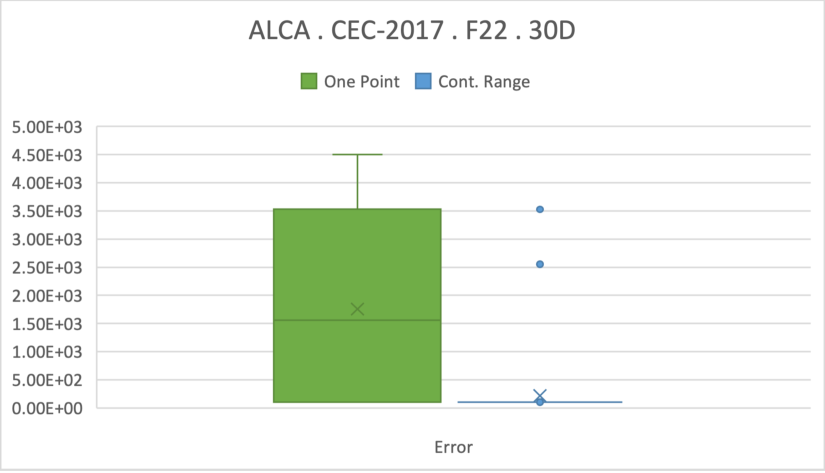
\includegraphics[width=1\linewidth]{img/fig_experiment_F22x30D.pdf} 
        \end{minipage}
        \vfill
        \vspace{0.05 cm}
        \begin{minipage}[h]{0.49\linewidth}
            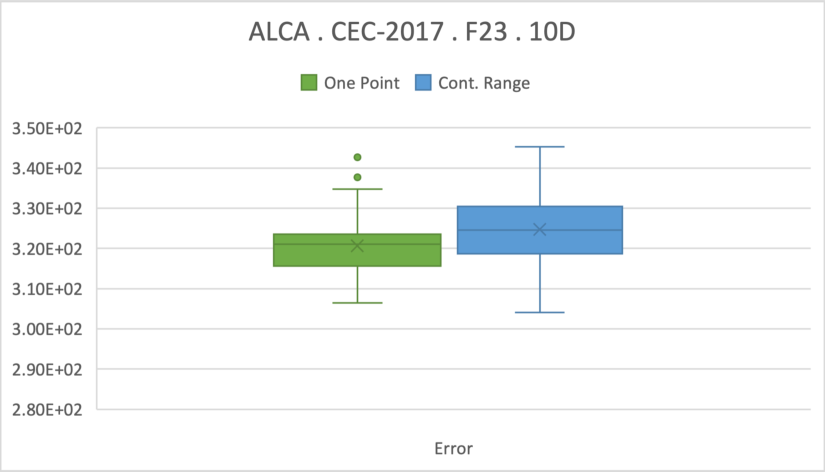
\includegraphics[width=1\linewidth]{img/fig_experiment_F23x10D.pdf} 
        \end{minipage}
        \hfill
        \begin{minipage}[h]{0.49\linewidth}
            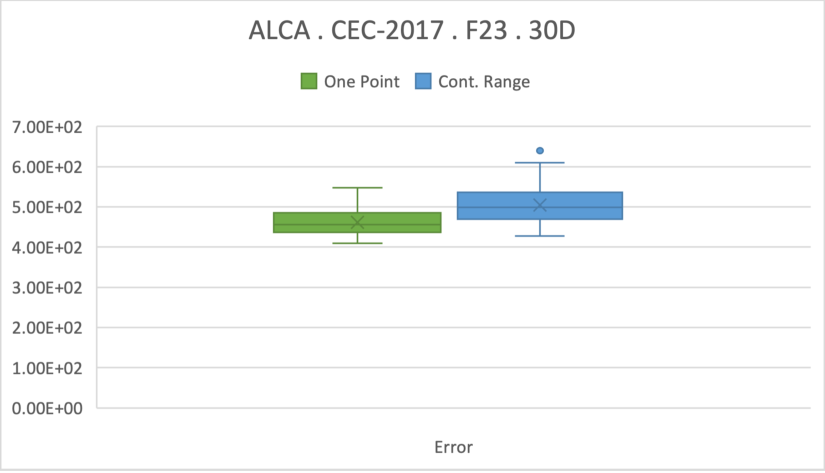
\includegraphics[width=1\linewidth]{img/fig_experiment_F23x30D.pdf} 
        \end{minipage}
        \vfill
        \vspace{0.05 cm}
        \begin{minipage}[h]{0.49\linewidth}
            \includegraphics[width=1\linewidth]{img/fig_experiment_F24x10D.pdf} 
        \end{minipage}
        \hfill
        \begin{minipage}[h]{0.49\linewidth}
            \includegraphics[width=1\linewidth]{img/fig_experiment_F24x30D.pdf} 
        \end{minipage}
        \vfill
        \vspace{0.05 cm}        
        \begin{minipage}[h]{0.49\linewidth}
            \includegraphics[width=1\linewidth]{img/fig_experiment_F25x10D.pdf} 
        \end{minipage}
        \hfill
        \begin{minipage}[h]{0.49\linewidth}
            \includegraphics[width=1\linewidth]{img/fig_experiment_F25x30D.pdf} 
        \end{minipage}
        
        \caption{Box and Whisker charts for mathematical functions F21 to F25. We display the ten and thirty-dimension charts on the left and right sides for the results accumulated in 51 runs.} \label{fig.experiment_F21-F25}
    \end{figure}

    \FloatBarrier

    \begin{figure}[!ht]
        \begin{minipage}[h]{0.49\linewidth}
            \includegraphics[width=1\linewidth]{img/fig_experiment_F26x10D.pdf} 
        \end{minipage}
        \hfill
        \begin{minipage}[h]{0.49\linewidth}
            \includegraphics[width=1\linewidth]{img/fig_experiment_F26x30D.pdf} 
        \end{minipage}
        \vfill
        \vspace{0.05 cm}
        \begin{minipage}[h]{0.49\linewidth}
            \includegraphics[width=1\linewidth]{img/fig_experiment_F27x10D.pdf} 
        \end{minipage}
        \hfill
        \vspace{0.05 cm}
        \begin{minipage}[h]{0.49\linewidth}
            \includegraphics[width=1\linewidth]{img/fig_experiment_F27x30D.pdf} 
        \end{minipage}
        \vfill
        \vspace{0.05 cm}
        \begin{minipage}[h]{0.49\linewidth}
            \includegraphics[width=1\linewidth]{img/fig_experiment_F28x10D.pdf} 
        \end{minipage}
        \hfill
        \begin{minipage}[h]{0.49\linewidth}
            \includegraphics[width=1\linewidth]{img/fig_experiment_F28x30D.pdf} 
        \end{minipage}
        \vfill
        \vspace{0.05 cm}
        \begin{minipage}[h]{0.49\linewidth}
            \includegraphics[width=1\linewidth]{img/fig_experiment_F29x10D.pdf} 
        \end{minipage}
        \hfill
        \begin{minipage}[h]{0.49\linewidth}
            \includegraphics[width=1\linewidth]{img/fig_experiment_F29x30D.pdf} 
        \end{minipage}
        \vfill
        \vspace{0.05 cm}
        \begin{minipage}[h]{0.49\linewidth}
            \includegraphics[width=1\linewidth]{img/fig_experiment_F30x10D.pdf} 
        \end{minipage}
        \hfill
        \begin{minipage}[h]{0.49\linewidth}
            \includegraphics[width=1\linewidth]{img/fig_experiment_F30x30D.pdf} 
        \end{minipage}        

        \caption{Box and Whisker charts for mathematical functions F26 to F30. We display the ten and thirty-dimension charts on the left and right sides for the results accumulated in 51 runs.} \label{fig.experiment_F26-F30}
    \end{figure}

    \FloatBarrier


% ---- Bibliography ----
% BibTeX users should specify bibliography style 'splncs04'.
% References will then be sorted and formatted in the correct style.
%

\bibliographystyle{splncs03_unsrt}
%\bibliographystyle{splncs04}
\bibliography{bib/bibliografia.bib}

\end{document}

% TO-DO: Turnitin.
